% !TeX root = ../thuthesis-example.tex

\chapter{测试驱动开发}

测试驱动开发(Test-Driven Development, TDD)是一种软件开发方法论,其核心思想是在编写实际功能代码之前先编写测试代码。这种"测试先行"的理念要求开发者首先定义预期行为和结果,然后才实现满足这些测试条件的功能代码。TDD的工作流程通常包括"红-绿-重构"三个阶段:首先编写一个失败的测试(红),然后编写最小可行的代码使测试通过(绿),最后对代码进行重构以改进设计(重构)\cite{Beck2002}。

bolt.se的测试功能模块是TDD理念在AI辅助开发环境中的创新实现,它允许用户创建和管理测试代码,并指导大语言模型(LLM)生成满足测试要求的代码。本章将详细介绍TDD的概念、意义、优势、对LLM驱动软件开发的重要性,以及bolt.se中测试功能的实现方案。

\section{测试驱动开发的概念与意义}

\subsection{TDD在软件工程中的优势}
测试驱动开发为现代软件工程带来了显著的优势:

\begin{enumerate}
  \item \textbf{设计优先}:TDD强制开发者在实现之前思考代码的接口和行为,促使更清晰的设计和更好的模块化。
  
  \item \textbf{快速反馈}:每次小的代码修改后立即运行测试,提供即时反馈,帮助开发者尽早发现问题。
  
  \item \textbf{回归保障}:完整的测试套件为代码重构和功能迭代提供安全网,确保新变更不会破坏现有功能。
  
  \item \textbf{文档作用}:测试代码自然地记录了系统预期行为和用例,成为活的文档,始终与代码保持同步。
  
  \item \textbf{专注与信心}:明确的测试目标帮助开发者保持专注,通过的测试提供信心,减少过度工程和不必要的复杂性。
\end{enumerate}

在bolt.se这样的现代开发平台中,这些优势得到了进一步放大,通过结构化的测试定义和自动化的测试执行,显著提升了开发效率和代码质量。

\subsection{TDD对LLM驱动软件开发的重要性}
在大型语言模型(LLM)驱动的软件开发范式中,测试驱动开发具有特殊且关键的意义\cite{Mathews2024}:

\begin{enumerate}
  \item \textbf{明确需求说明}:测试用例为LLM提供了清晰、结构化的需求描述,减少了需求理解的模糊性和误解。
  
  \item \textbf{引导代码生成}:测试代码明确了预期行为,为LLM提供了具体目标,引导它生成满足特定功能和质量要求的代码。
  
  \item \textbf{减少幻觉和错误}:确定的测试约束降低了LLM生成不准确或幻想代码的可能性,因为生成的代码必须通过测试验证。
  
  \item \textbf{可验证性保证}:测试提供了自动化的验证机制,确保LLM生成的代码实际上能够正确运行,而非仅看起来合理。
  
  \item \textbf{迭代优化基础}:测试结果为LLM提供结构化反馈,使其能够针对性地改进代码,实现持续优化。
\end{enumerate}

在bolt.se中,TDD理念已经深度融入系统设计。通过将测试代码集成到对话上下文中,bolt.se实现了LLM与测试用例的无缝协作,使开发者能够通过自然语言交互获得测试驱动的智能编码辅助。这种结合保留了LLM的创造力和灵活性,同时增加了可靠性和正确性保证,为软件开发带来了质的飞跃。

\section{Jest测试框架与TDD实践}

Jest是一个由Facebook开发的JavaScript测试框架,专注于简单性和易用性,已成为前端测试的流行选择\cite{Jest2023}。bolt.se采用Jest作为其测试功能的核心框架,充分利用其强大的特性支持TDD实践。

\subsection{Jest测试框架简介}

Jest提供了全面的测试解决方案,具有以下主要特性:

\begin{enumerate}
  \item \textbf{零配置测试平台}:默认包含断言库、测试运行器、模拟工具等,减少配置负担。
  
  \item \textbf{描述性API}:通过describe、it/test、expect等函数提供表达力强的测试API,使测试代码易于理解和维护。
  
  \item \textbf{快照测试}:支持UI组件和数据结构的快照比对,简化回归测试。
  
  \item \textbf{丰富的匹配器}:提供多种断言方法,适应不同的测试需求。
  
  \item \textbf{并行测试执行}:默认并行运行测试,提高效率。
  
  \item \textbf{代码覆盖率报告}:内置覆盖率收集和报告功能。
\end{enumerate}

在bolt.se中,Jest测试通常采用以下结构:

\begin{verbatim}
// 测试套件
describe('Calculator', () => {
  // 测试用例
  test('adds 1 + 2 to equal 3', () => {
    expect(add(1, 2)).toBe(3);
  });
  
  test('subtracts 5 - 2 to equal 3', () => {
    expect(subtract(5, 2)).toBe(3);
  });
});
\end{verbatim}

bolt.se的测试功能模块能够解析这种Jest测试结构,自动提取测试套件和测试用例,呈现给用户,并引导LLM生成满足测试要求的代码。

\subsection{TDD的实践方法与工作流程}

在bolt.se环境中,TDD实践遵循特定的工作流程,融合了传统TDD与AI辅助开发的优势:

\begin{enumerate}
  \item \textbf{测试编写}:用户在bolt.se的测试编辑器中创建测试代码,描述期望的功能行为。
  
  \item \textbf{测试解析与结构化}:系统自动解析测试代码,提取测试套件和测试用例的结构,以可视化树形结构展示。
  
  \item \textbf{测试注入对话}:用户开始新对话时,系统将测试代码作为上下文信息注入给LLM。
  
  \item \textbf{指导代码生成}:LLM根据测试用例理解需求,生成满足测试条件的实现代码。
  
  \item \textbf{测试执行与验证}:用户可以一键运行测试,验证生成代码是否通过所有测试。
  
  \item \textbf{迭代改进}:根据测试结果,用户可以要求LLM修改代码,或调整测试用例,进入新的开发周期。
\end{enumerate}

这种工作流程使传统TDD的优势与AI辅助开发的效率相结合,为开发者提供了前所未有的开发体验。

\section{bolt.se中的测试功能实现}

bolt.se作为一个AI驱动的软件开发平台,将TDD理念深度融入其架构设计。系统通过结构化的测试功能模块,使用户能够轻松创建、管理和应用测试代码,同时让大语言模型能够理解并满足这些测试要求,实现高质量的代码生成。本节将详细介绍bolt.se中测试功能的实现方案,从整体架构设计到具体功能实现。

\begin{figure}[htbp]
  \centering
  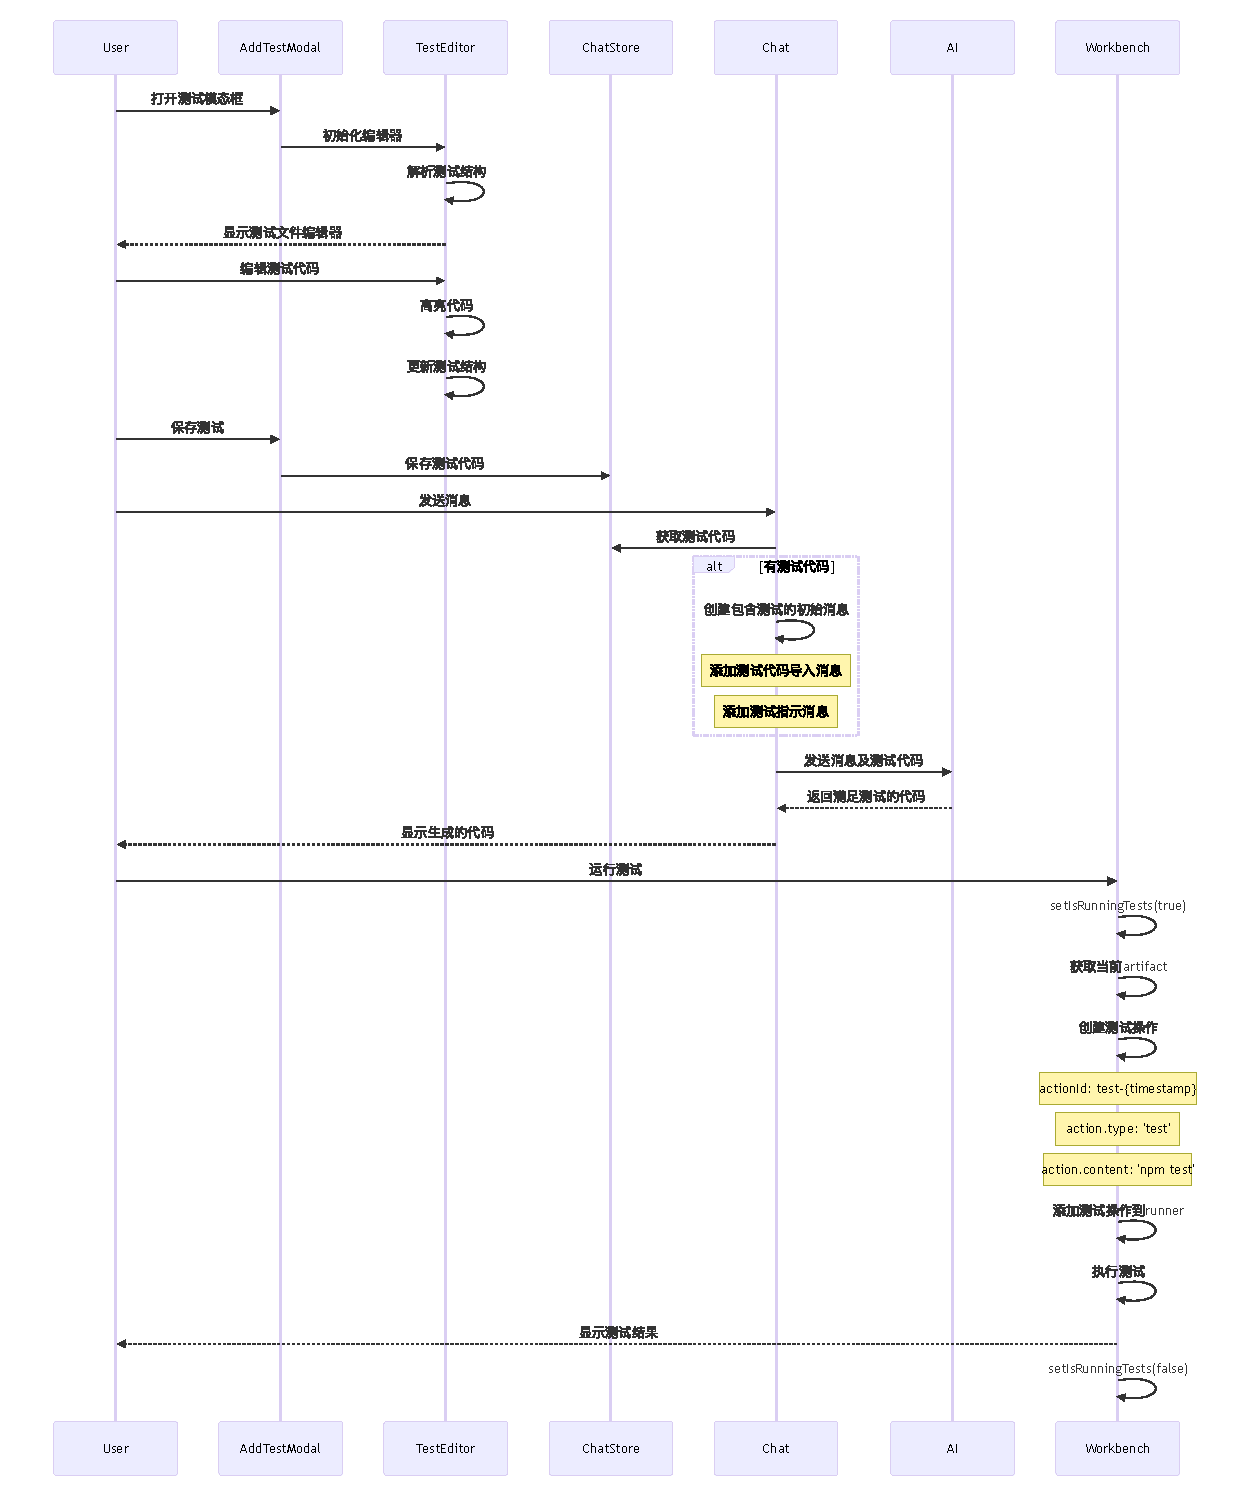
\includegraphics[width=\textwidth]{figures/bolt_test_sequence.pdf}
  \caption{测试功能流程图:展示了用户创建、编辑和使用测试的完整流程,以及测试信息如何在系统各组件间传递}
  \label{fig:test_sequence}
\end{figure}

\subsection{整体架构设计与模块划分}

bolt.se的测试系统采用了模块化设计,主要由以下几个核心组件构成:

\begin{enumerate}
  \item \textbf{用户界面组件}:
    \begin{itemize}
      \item \texttt{AddTestModal}:管理测试的主要模态窗口,支持创建和编辑测试代码
      \item \texttt{TestEditor}:测试代码的编辑器组件,提供语法高亮和结构可视化
      \item \texttt{TestStructure}:递归渲染测试树的组件,展示测试套件和测试用例的层次关系
    \end{itemize}
  
  \item \textbf{数据管理组件}:
    \begin{itemize}
      \item \texttt{chatStore}:管理当前聊天中的测试代码(testCodes)
      \item \texttt{IndexedDB存储}:持久化存储测试定义
    \end{itemize}
  
  \item \textbf{测试执行组件}:
    \begin{itemize}
      \item \texttt{Workbench}:提供测试运行环境
      \item \texttt{ActionRunner}:负责执行测试命令并收集结果
    \end{itemize}
  
  \item \textbf{AI交互层}:负责将测试代码传递给大语言模型,并处理模型的响应结果
\end{enumerate}

如图\ref{fig:test_sequence}所示,整个测试使用流程分为三个主要阶段:测试创建与编辑、在对话中使用测试引导代码生成,以及测试执行与验证。这种设计确保了测试的全生命周期管理,从定义到使用再到验证的完整闭环。

在数据模型设计方面,bolt.se定义了结构化的测试数据模型,如图\ref{fig:test_class}所示。核心数据结构包括TestCodeItem、TestItem、TestCase和TestSuite:

\begin{figure}[htbp]
  \centering
  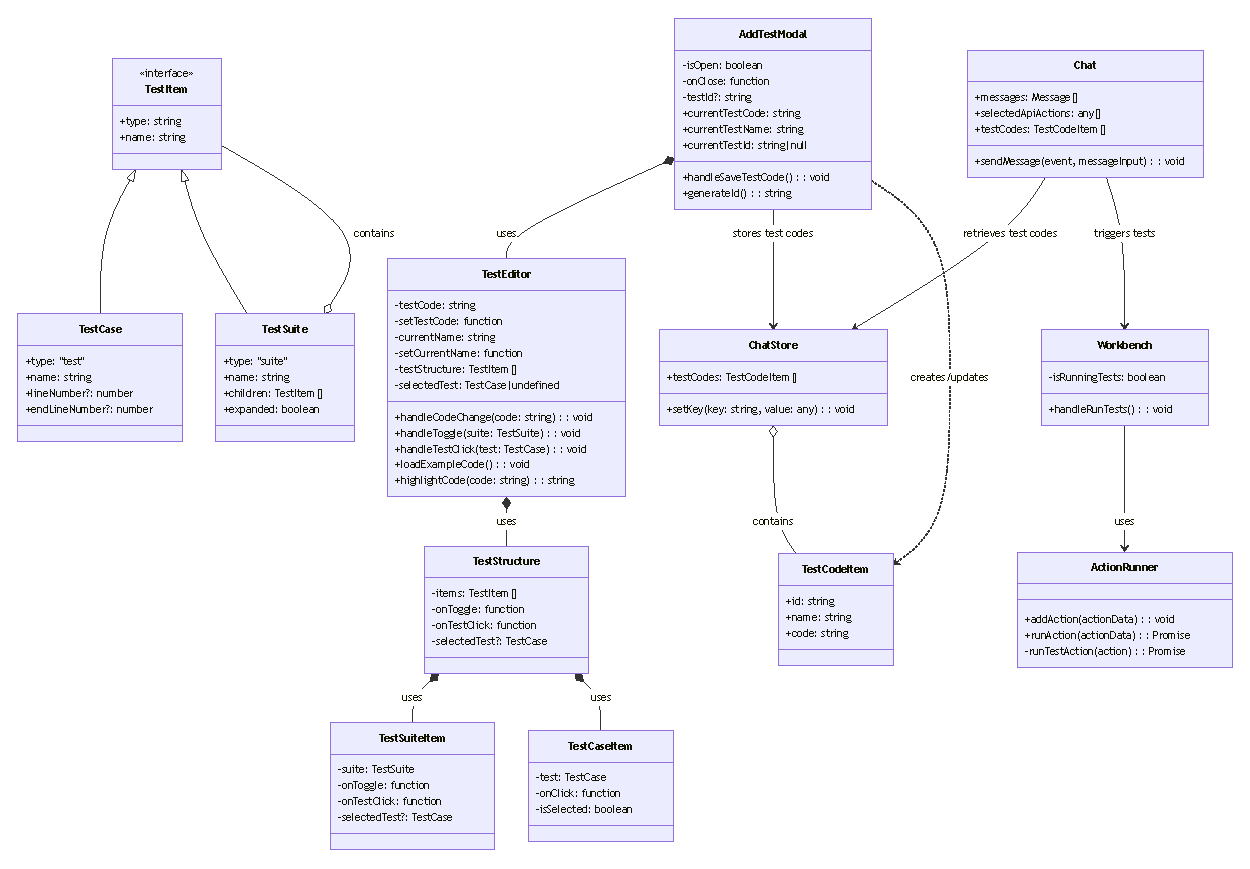
\includegraphics[width=\textwidth]{figures/bolt_test_class.pdf}
  \caption{测试数据模型类图:描述了系统中测试定义的核心数据结构及其关系,包括测试代码项、测试用例、测试套件和用户界面组件}
  \label{fig:test_class}
\end{figure}

测试数据模型的主要组成包括:

\begin{enumerate}
  \item \textbf{TestCodeItem}:表示一个测试文件,包含唯一标识符(id)、名称(name)和测试代码(code)。
  
  \item \textbf{TestItem}:测试项的接口,是TestCase和TestSuite的基类,包含类型(type)和名称(name)。
  
  \item \textbf{TestCase}:表示具体的测试用例,包含类型("test")、名称和在代码中的行号范围。
  
  \item \textbf{TestSuite}:表示测试套件,包含类型("suite")、名称、子测试项数组和展开状态。
\end{enumerate}

bolt.se的测试功能模块具有以下关键功能:

\begin{enumerate}
  \item \textbf{测试代码解析}:系统能够解析Jest测试代码,自动识别并提取测试套件和测试用例,构建树形结构。
  
  \item \textbf{测试代码编辑器}:提供语法高亮和结构可视化的专用编辑器,支持测试代码的创建和编辑。
  
  \item \textbf{测试导入对话}:自动将测试代码转换为文件操作指令,注入到对话中,作为上下文提供给LLM。
  
  \item \textbf{测试执行机制}:通过Workbench组件提供一键测试执行功能,验证生成代码是否满足测试要求。
  
  \item \textbf{测试结果反馈}:收集并展示测试执行结果,便于用户了解代码质量和问题所在。
\end{enumerate}

\subsection{测试解析与可视化}

bolt.se实现了强大的测试代码解析和可视化功能,帮助用户更直观地理解和管理测试:

\begin{enumerate}
  \item \textbf{正则表达式解析}:使用正则表达式识别测试代码中的describe和it/test函数调用,提取测试套件和测试用例的名称。
  
  \item \textbf{语法树构建}:根据代码缩进和嵌套关系,构建测试的层次结构,形成树形数据模型。
  
  \item \textbf{位置追踪}:记录每个测试用例在代码中的起始和结束行号,便于导航和高亮显示。
  
  \item \textbf{交互式树形视图}:将解析结果以可折叠的树形结构展示,支持测试套件的展开和折叠。
  
  \item \textbf{代码高亮与定位}:点击测试用例时,自动高亮显示对应的代码区域,并滚动到可见位置。
\end{enumerate}

这些功能大大提升了测试代码的可读性和可维护性,使用户能够更高效地管理复杂的测试套件。

\subsection{测试与LLM集成机制}

bolt.se创新性地将测试与LLM集成,实现了测试驱动的AI辅助开发:

\begin{enumerate}
  \item \textbf{测试注入}:当用户开始新对话时,系统自动将选定的测试代码转换为文件操作指令,注入到对话上下文中。
  
  \item \textbf{指导消息}:系统生成专门的指导消息,告知LLM需要生成满足测试要求的代码,并提供具体步骤。
  
  \item \textbf{环境准备引导}:指导LLM安装必要的依赖,配置测试脚本,准备测试环境。
  
  \item \textbf{测试执行提示}:建议LLM在开发服务器启动前运行测试,验证代码正确性。
  
  \item \textbf{错误修复循环}:测试失败时,用户可以将错误信息反馈给LLM,引导其修复问题,形成迭代改进循环。
\end{enumerate}

这种集成机制使LLM能够理解并遵循TDD原则,生成高质量、符合预期的代码,同时提供了验证机制确保代码的正确性。

\section{实例应用场景}

本节通过一个实际开发示例,展示如何在bolt.se中使用测试驱动开发功能,从测试编写到代码生成,再到测试验证的完整流程。

\subsection{创建和编辑测试}

用户首先通过AddTestModal创建测试代码,如图所示,编写一个简单的计算器功能测试:

\begin{verbatim}
describe('Calculator', () => {
  test('adds 1 + 2 to equal 3', () => {
    const { add } = require('../calculator');
    expect(add(1, 2)).toBe(3);
  });
  
  test('subtracts 5 - 2 to equal 3', () => {
    const { subtract } = require('../calculator');
    expect(subtract(5, 2)).toBe(3);
  });
  
  test('multiplies 2 * 3 to equal 6', () => {
    const { multiply } = require('../calculator');
    expect(multiply(2, 3)).toBe(6);
  });
  
  test('divides 6 / 2 to equal 3', () => {
    const { divide } = require('../calculator');
    expect(divide(6, 2)).toBe(3);
  });
});
\end{verbatim}

系统自动解析这些测试,提取测试套件"Calculator"和四个测试用例,在左侧面板以树形结构展示。

\subsection{使用测试引导代码生成}

创建测试后,用户开始新对话并提交需求:

\begin{quote}
\texttt{根据测试要求,实现一个简单的计算器模块}
\end{quote}

系统自动将测试代码作为上下文注入对话,并生成指导消息告知LLM:

\begin{quote}
\texttt{一个测试文件已被导入用于vitest。你需要确保生成的代码通过测试,通过:\\
- 安装必要的依赖\\
- 添加"test": "vitest run"脚本到package.json\\
- 导入测试文件所需的函数\\
- 在启动开发服务器前执行测试验证所有测试通过}
\end{quote}

LLM理解测试要求,生成满足条件的计算器模块实现:

\begin{verbatim}
// calculator.js
exports.add = (a, b) => a + b;
exports.subtract = (a, b) => a - b;
exports.multiply = (a, b) => a * b;
exports.divide = (a, b) => a / b;
\end{verbatim}

同时生成package.json和测试配置:

\begin{verbatim}
// package.json
{
  "name": "calculator",
  "version": "1.0.0",
  "scripts": {
    "test": "vitest run"
  },
  "devDependencies": {
    "vitest": "^0.34.3"
  }
}
\end{verbatim}

\subsection{测试执行与验证}

用户可以通过Workbench中的"Run Tests"按钮执行测试,验证生成的代码\cite{Vitest2023}:

\begin{verbatim}
$ npm test

> calculator@1.0.0 test
> vitest run

✓ __test__/calculator_test.test.js (4 tests) 3ms
  ✓ Calculator (4 tests) 3ms
    ✓ adds 1 + 2 to equal 3 1ms
    ✓ subtracts 5 - 2 to equal 3 0ms
    ✓ multiplies 2 * 3 to equal 6 0ms
    ✓ divides 6 / 2 to equal 3 0ms

Test Files  1 passed (1)
Tests       4 passed (4)
Start at    20:45:32
Duration    1.20s (transform 115ms, setup 0ms, collect 15ms, tests 3ms)
\end{verbatim}

测试全部通过,证明生成的代码满足了测试要求。如果有测试失败,用户可以将错误信息提供给LLM,引导其修复问题。

\section{TDD与传统开发方式对比}

TDD在bolt.se中的实现与传统开发方式相比具有显著优势:

\begin{enumerate}
  \item \textbf{需求明确性}:传统方法中,开发者需要从自然语言描述中理解需求,而TDD方法通过具体的测试代码明确定义了预期行为,减少了理解偏差。
  
  \item \textbf{开发效率}:在bolt.se的TDD模式下,LLM能够直接从测试理解需求并生成符合要求的代码,避免了反复沟通和解释需求的过程。
  
  \item \textbf{代码质量}:测试驱动的代码生成确保了每个功能都有对应的测试覆盖,自然形成高测试覆盖率,提高了代码质量和可靠性。
  
  \item \textbf{反馈速度}:即时的测试执行提供了快速反馈,使开发者能够立即知道代码是否符合预期,加速了开发迭代。
  
  \item \textbf{文档价值}:测试代码自然成为系统功能的活文档,比传统注释和文档更准确、更容易保持同步。
\end{enumerate}

特别是在LLM辅助开发环境中,TDD的优势被进一步放大:

\begin{enumerate}
  \item \textbf{减少幻觉}:结构化的测试要求降低了LLM生成错误或幻想代码的可能性,因为所有代码都必须通过测试验证。
  
  \item \textbf{引导性强}:测试代码为LLM提供了明确的目标和约束,使其生成的代码更符合实际需求。
  
  \item \textbf{验证机制}:测试提供了客观的验证标准,避免了仅凭代码外观判断质量的主观性。
  
  \item \textbf{迭代基础}:测试结果为LLM提供了结构化反馈,使其能够有针对性地改进代码。
\end{enumerate}

这些优势使得TDD成为bolt.se中AI辅助开发的理想方法论,提供了高效、高质量的开发体验。

\section{实例应用场景}
\label{sec:tdd-example}

本节通过 JavaScript 计算器的完整开发流程,说明在 bolt.se 中如何围绕
“红–绿–重构”循环进行测试驱动开发,并借助大语言模型完成自动修复与演进。

\subsection{插入 Jest 测试代码与需求声明}

\begin{figure}[htbp]
  \centering
  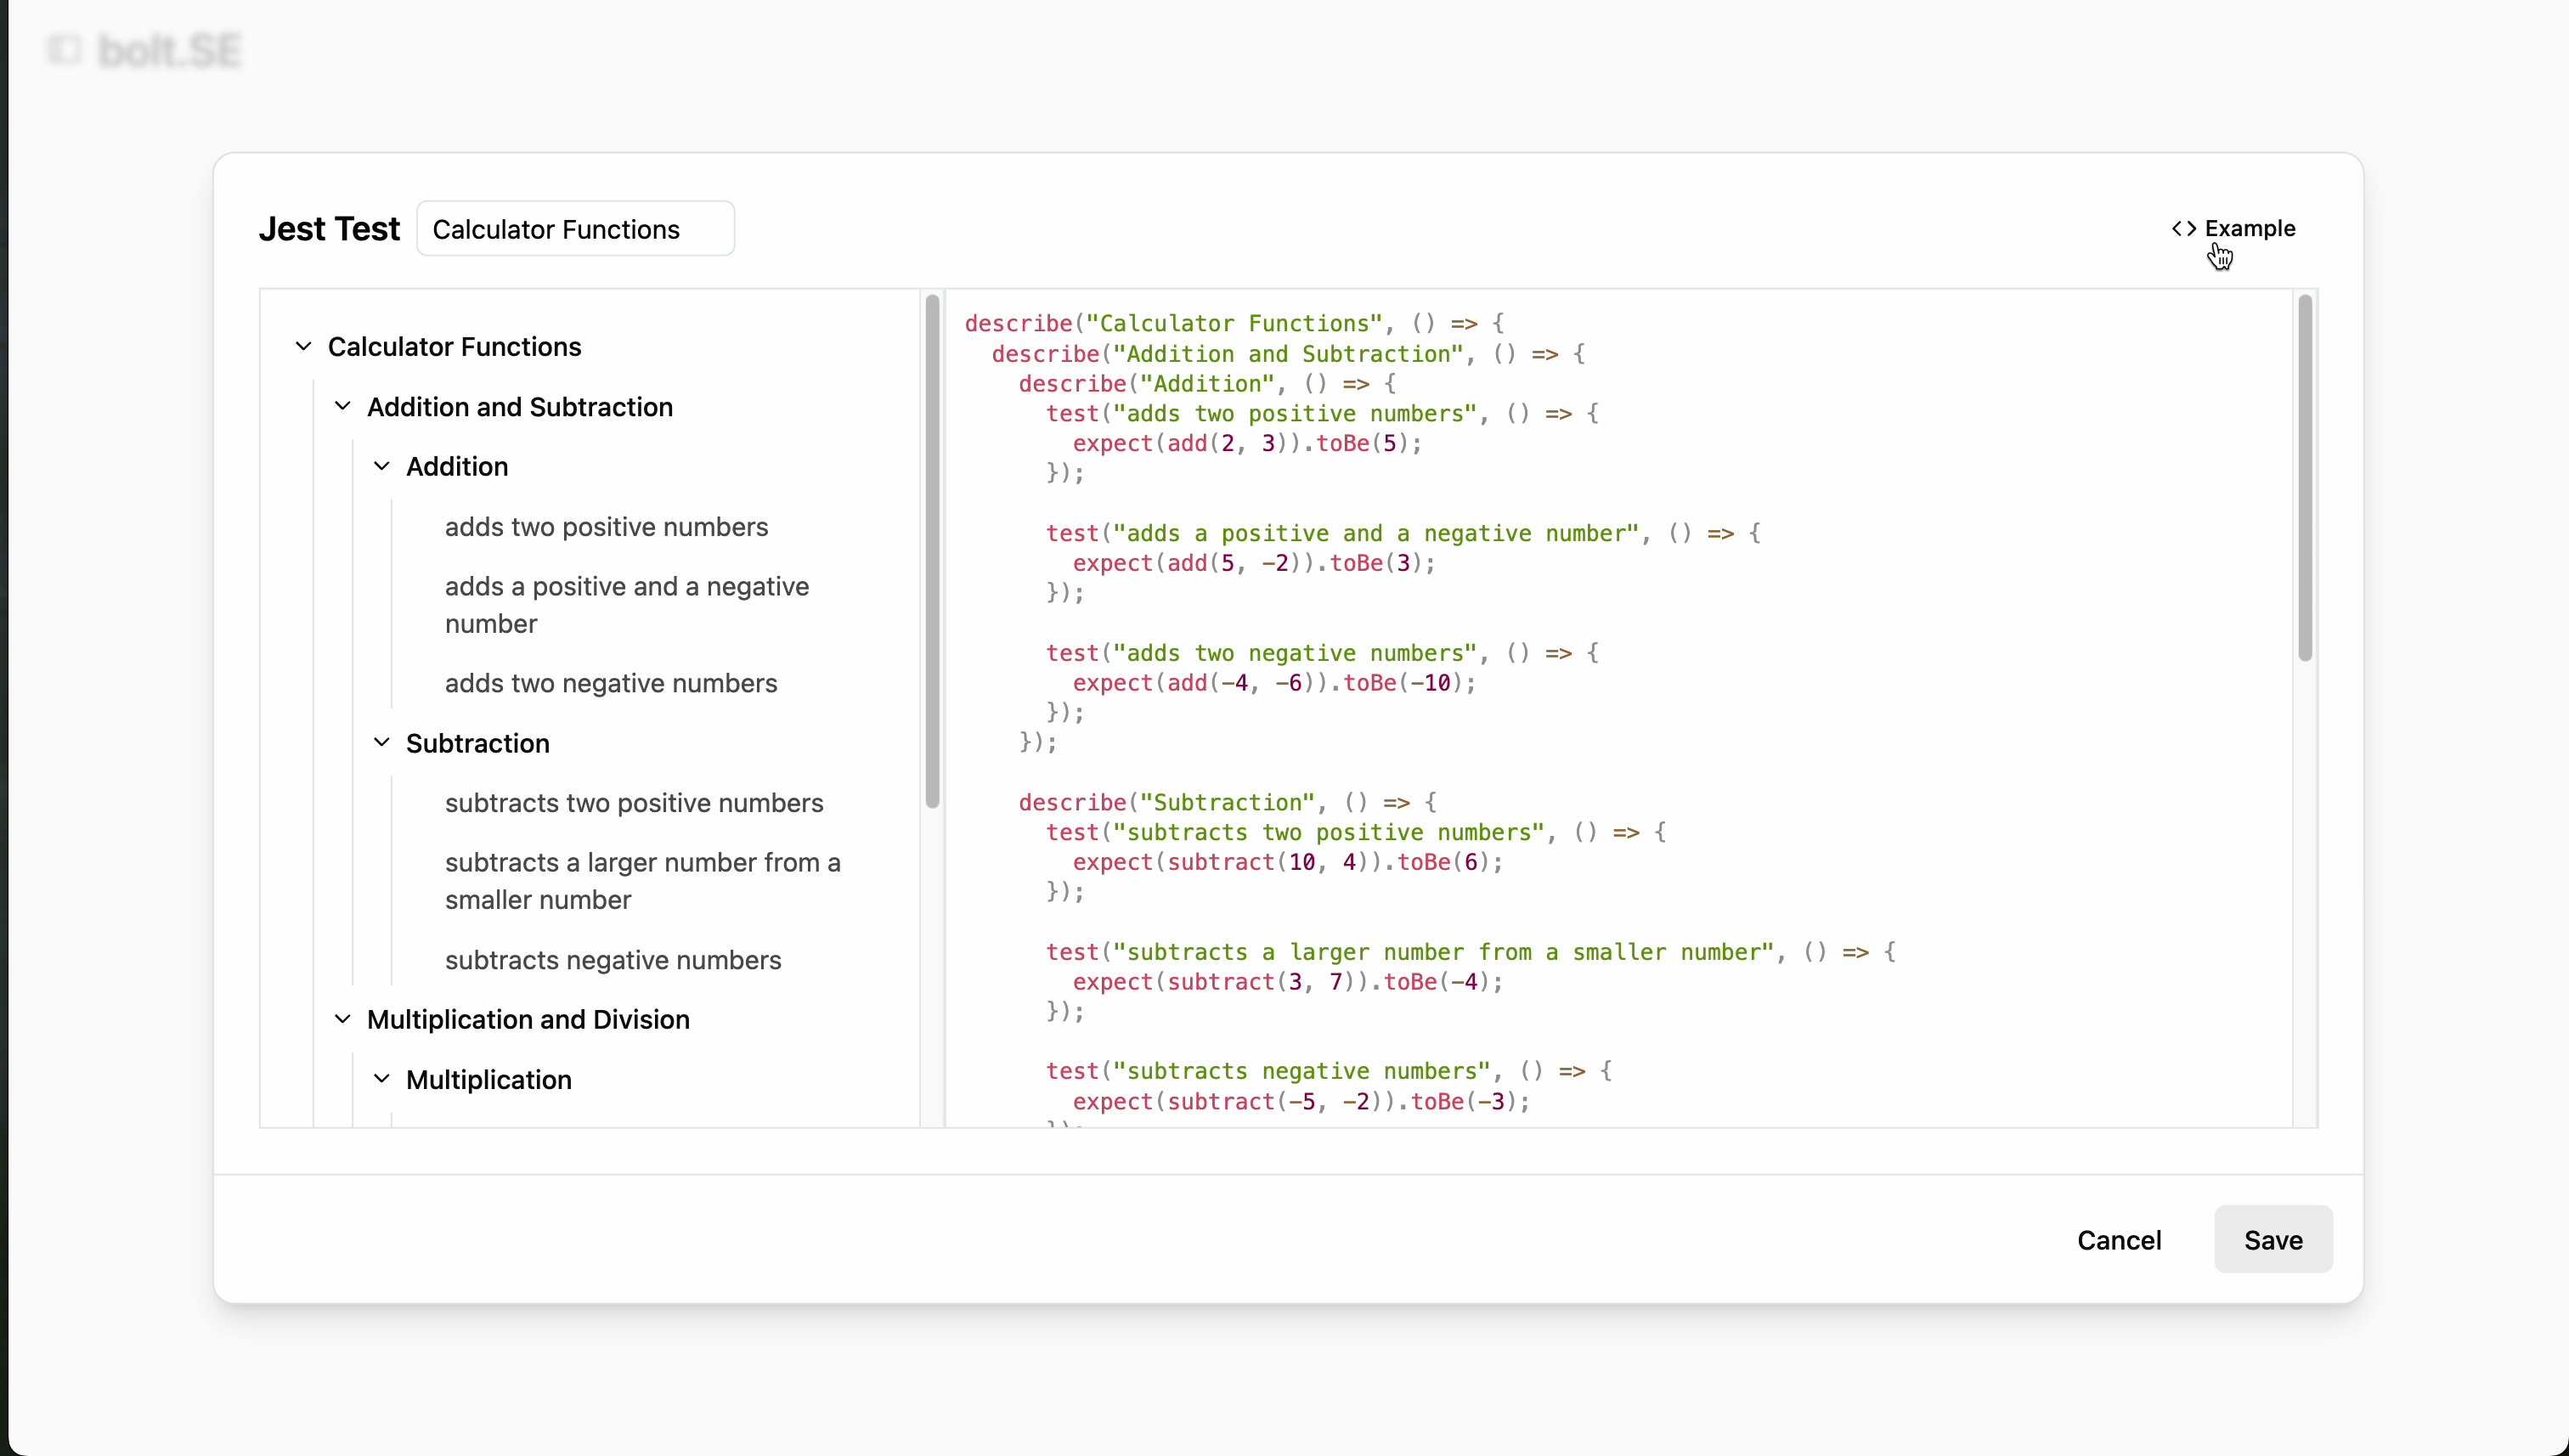
\includegraphics[width=.9\textwidth]{figures/screenshots/tdd/add_test_modal.png}
  \caption{在 AddTestModal 中粘贴 \texttt{calculator\_functions.test.js}。
           系统解析出 \textit{Calculator Functions} 测试套件与 12 条断言,
           以树形结构展示。}
  \label{fig:tdd_add_test}
\end{figure}

开发者首先将一组覆盖加、减、乘、除等核心功能的测试用例粘贴至测试编辑器,
bolt.se 立即完成以下操作:

\begin{enumerate}
  \item 解析 \verb|describe| 与 \verb|test| 调用,构建测试树;
  \item 将测试文件保存在项目目录,并写入 IndexedDB 以便持久化;
  \item 在对话上下文中注册该文件,供后续提示使用。
\end{enumerate}

\begin{figure}[htbp]
  \centering
  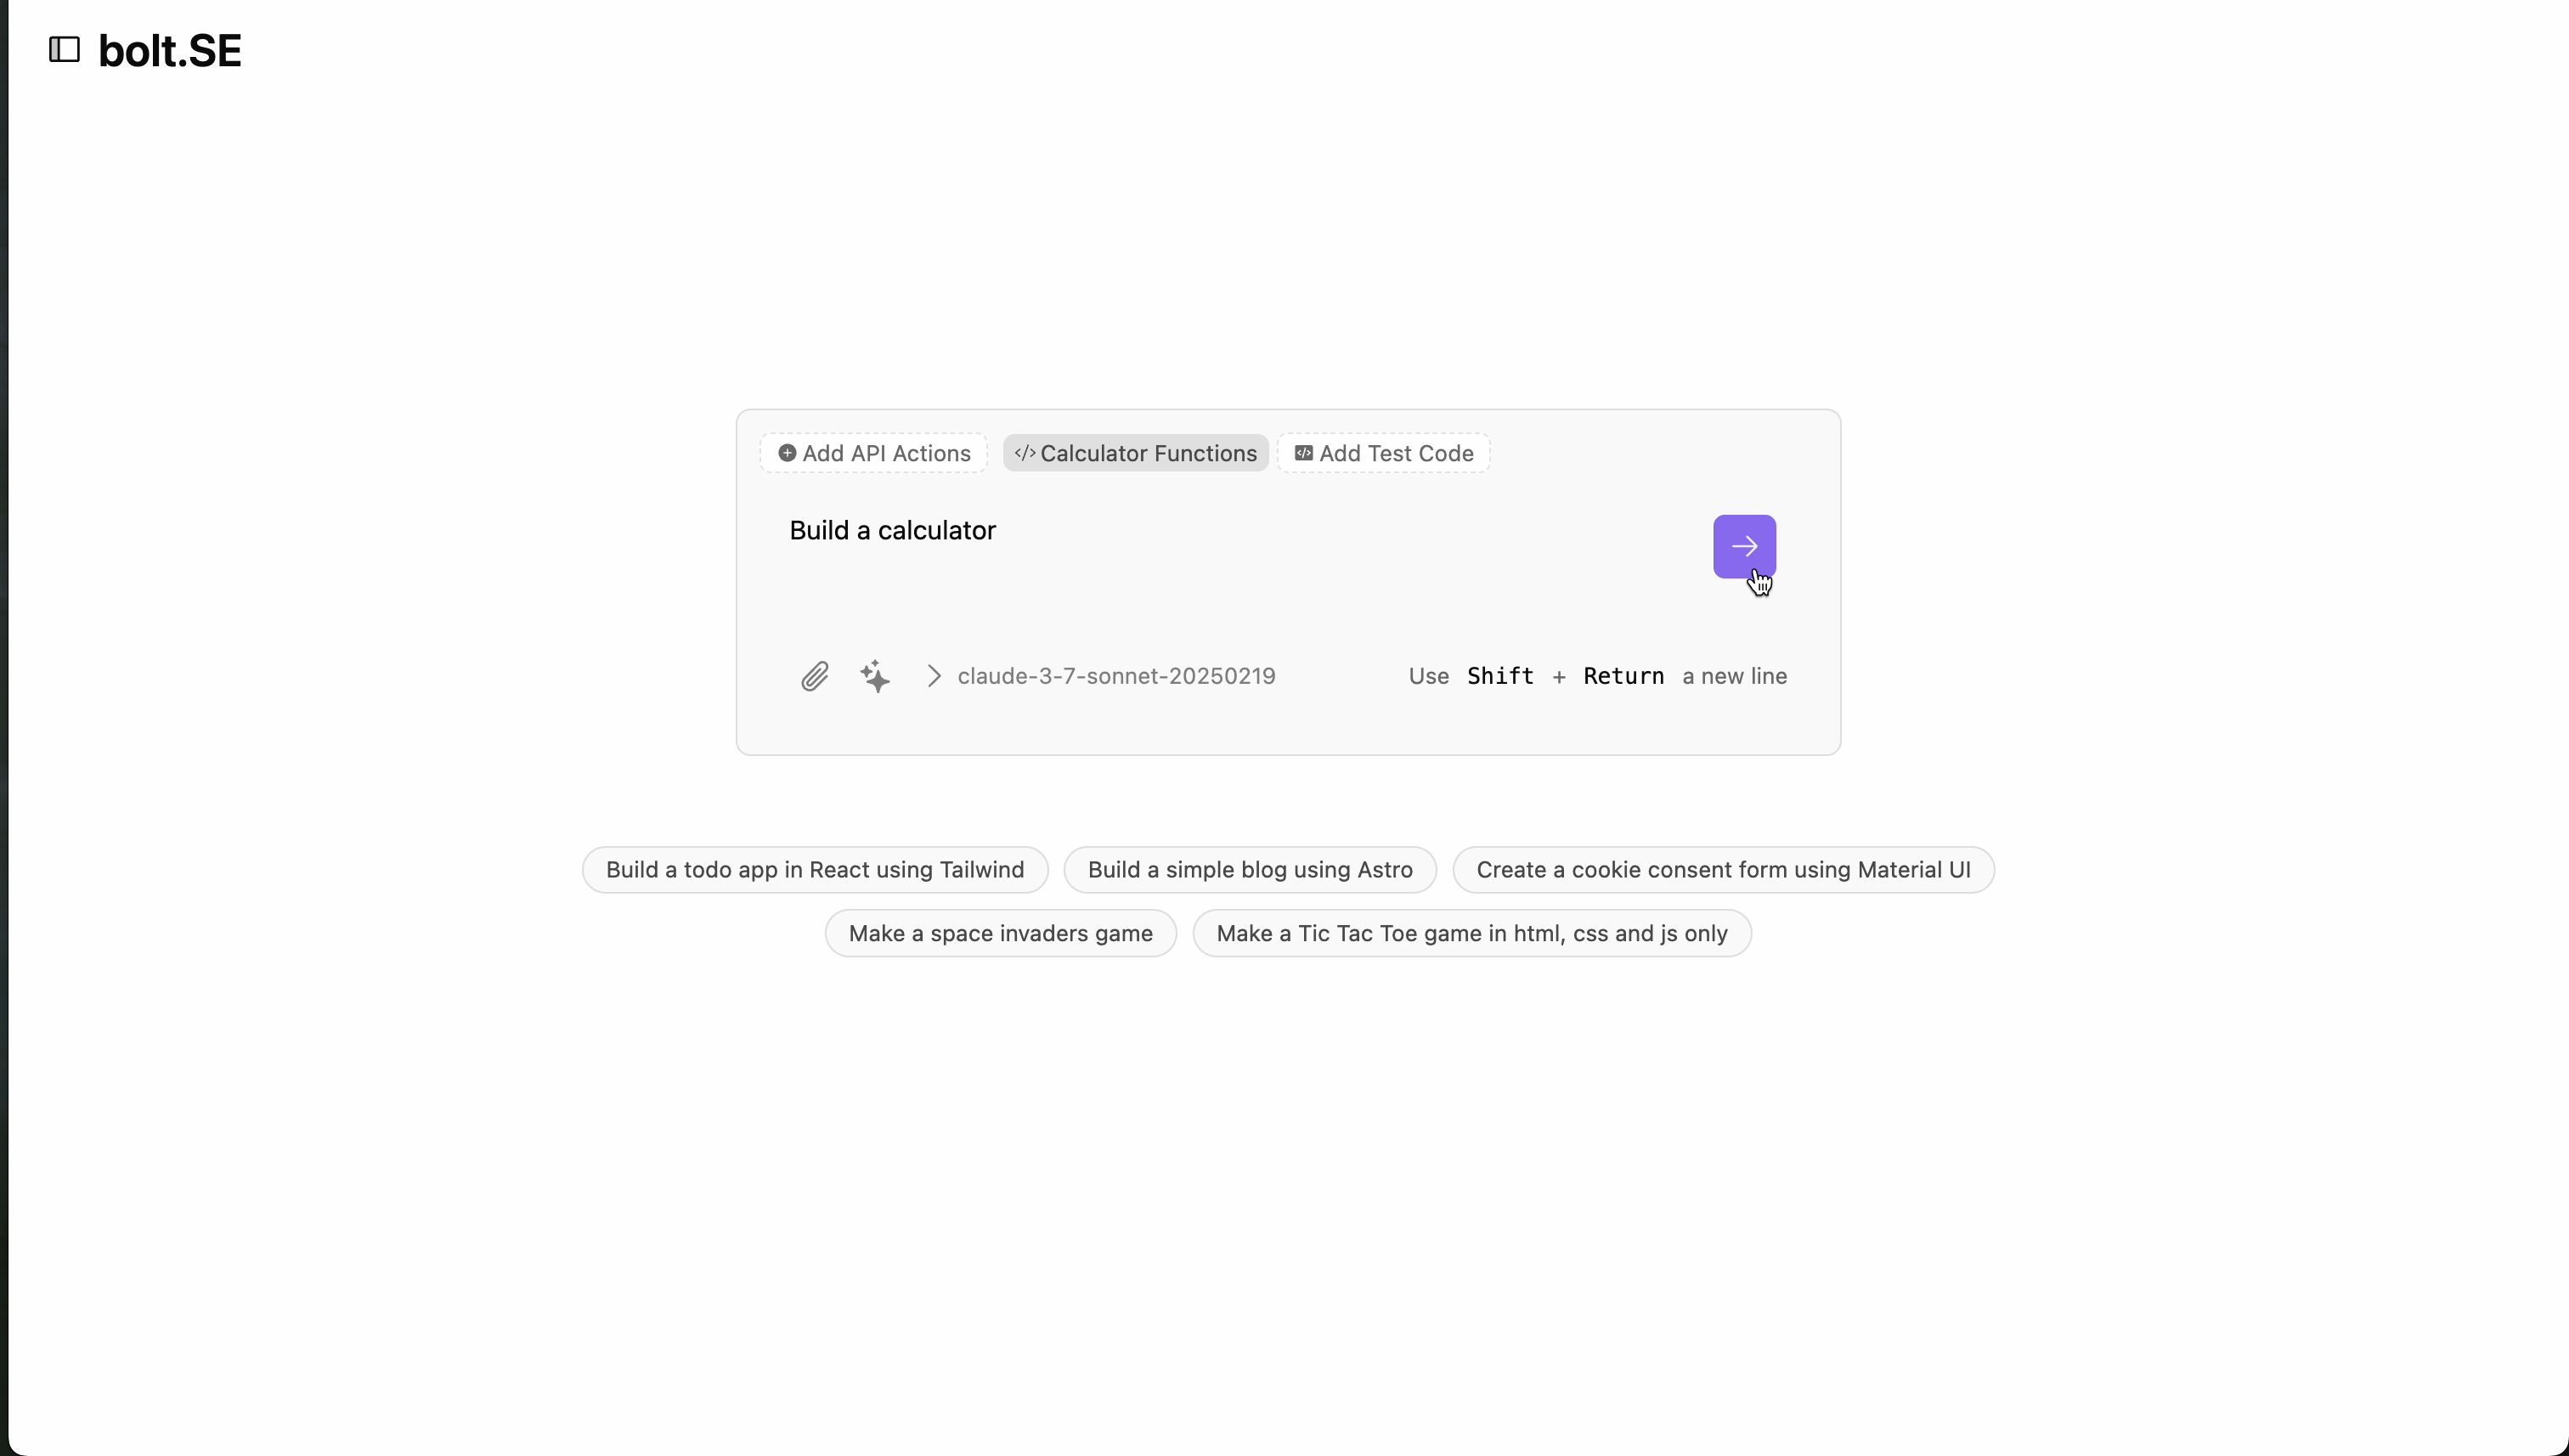
\includegraphics[width=.9\textwidth]{figures/screenshots/tdd/calculator_prompt.png}
  \caption{随后在聊天窗口输入自然语言需求
           “Build a calculator”。系统自动把测试文件和指导语注入同一条提示,
           为 LLM 提供明确的功能规格。}
  \label{fig:tdd_prompt}
\end{figure}

\subsection{首次执行——绿灯}

\begin{figure}[htbp]
  \centering
  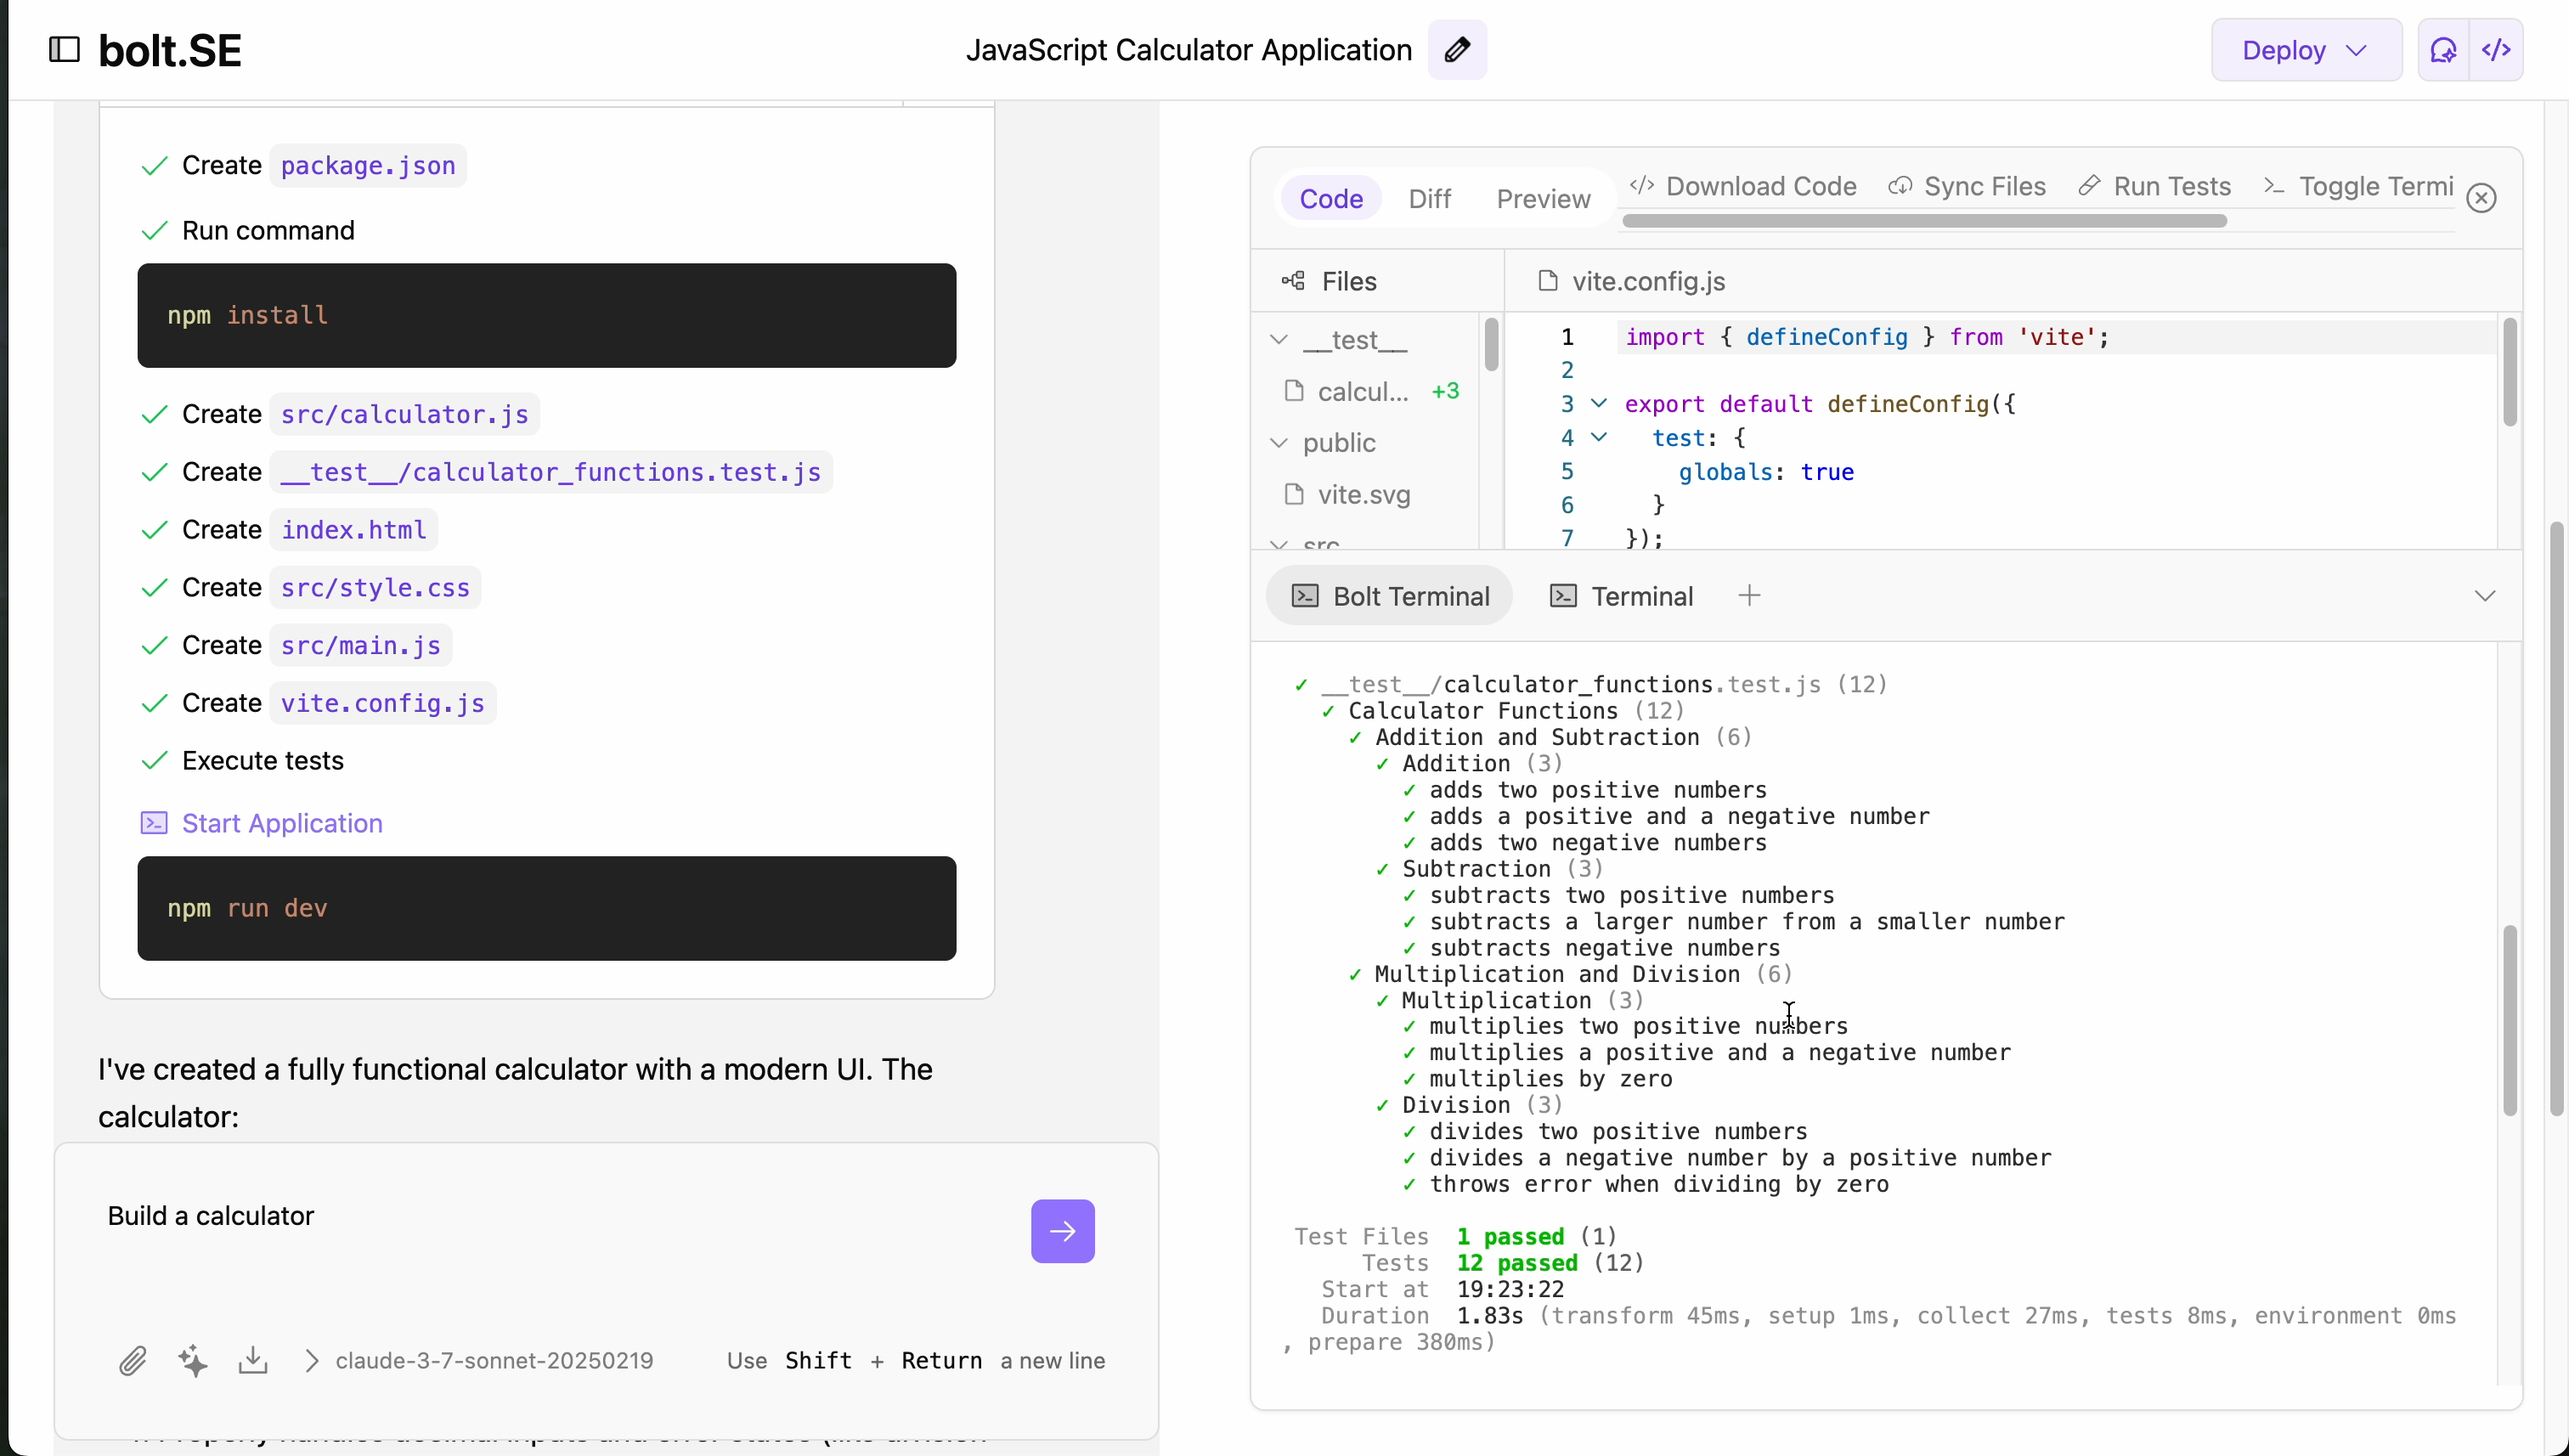
\includegraphics[width=.9\textwidth]{figures/screenshots/tdd/green_pass_initial.png}
  \caption{LLM 依据测试生成 \texttt{calculator.js} 等文件。
           运行 Vitest 后 12 条断言全部通过,终端显示绿灯状态。}
  \label{fig:tdd_green_initial}
\end{figure}

LLM 读取测试用例后,创建四个算术函数并配置
\verb|"test": "vitest run"|。  
统一通过的结果表明当前实现满足原始规格。

\subsection{引入红灯:提高规格造成断言失败}

为演示迭代过程,开发者手动把其中一条加法断言改为
\verb|expect(add(2, 3)).toBe(0);|,等价于提出“2 + 3 需要返回 0”这一
不合常理但更严格的新需求。

\begin{figure}[htbp]
  \centering
  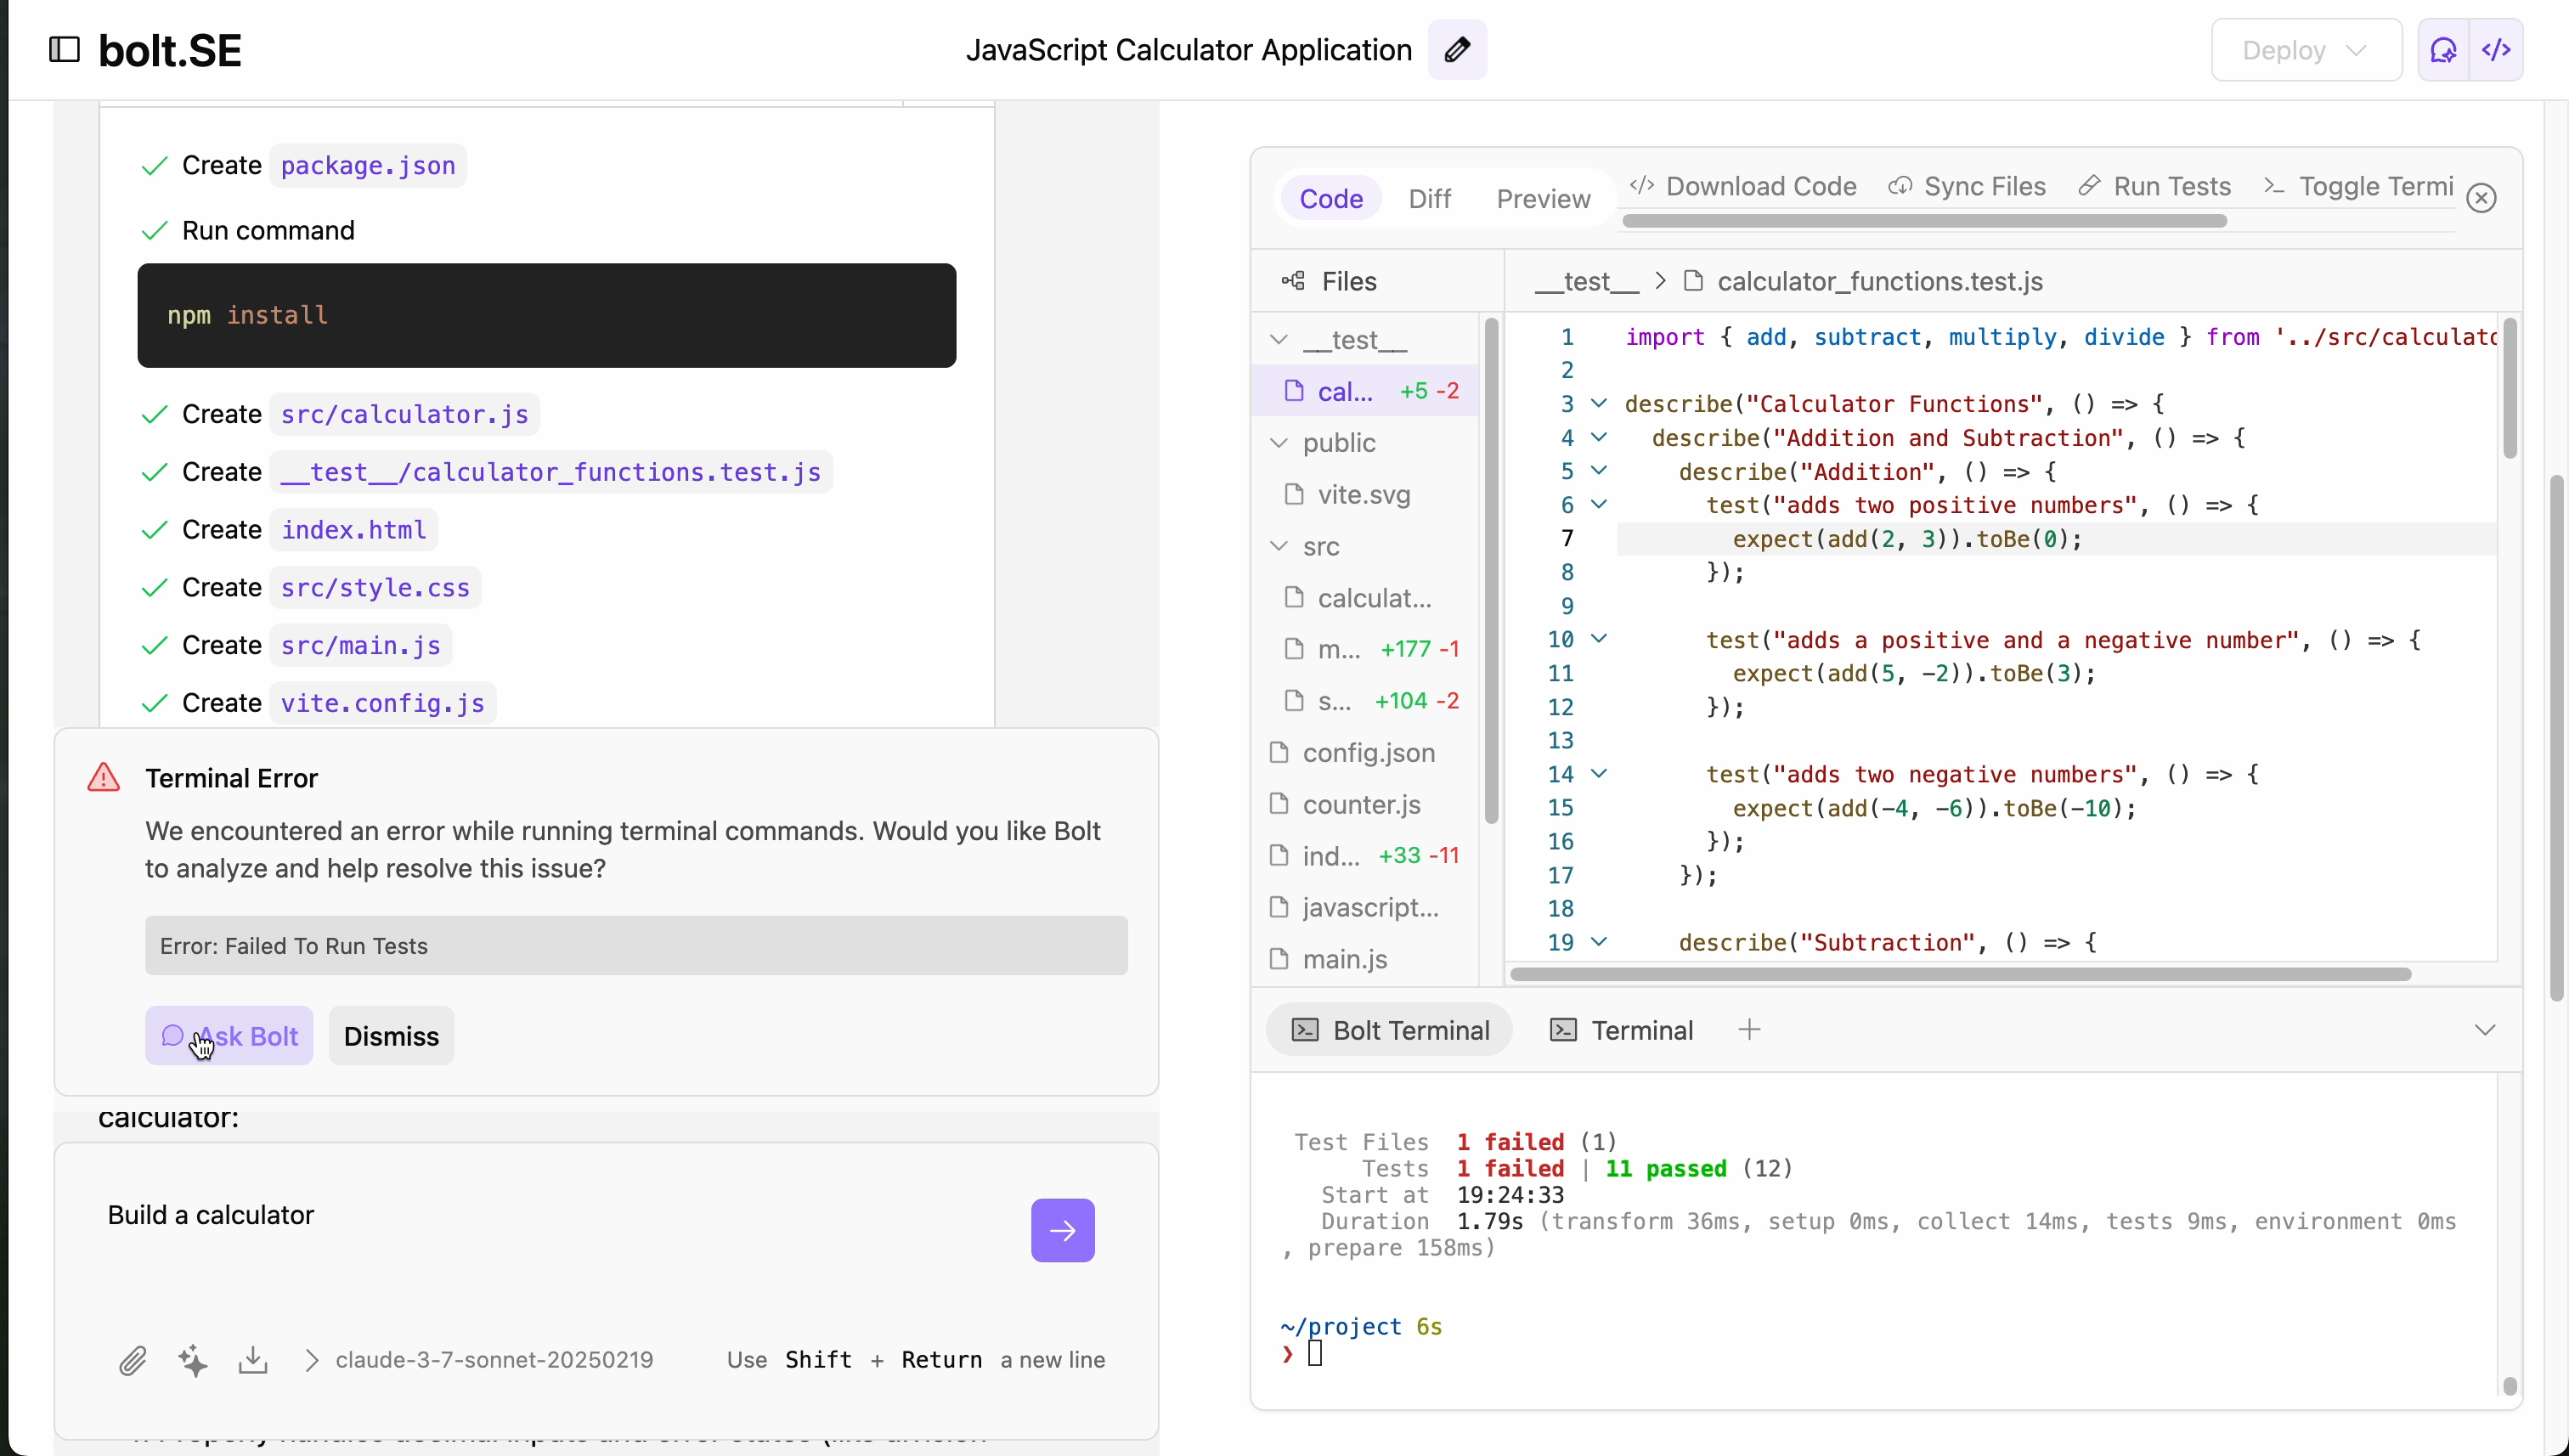
\includegraphics[width=.9\textwidth]{figures/screenshots/tdd/test_edit_fail.png}
  \caption{修改断言后再次运行测试,出现 1 条失败记录。  
           终端输出红色标记,进入红灯阶段。}
  \label{fig:tdd_red}
\end{figure}

\subsection{模型修复——重新转绿}

\begin{figure}[htbp]
  \centering
  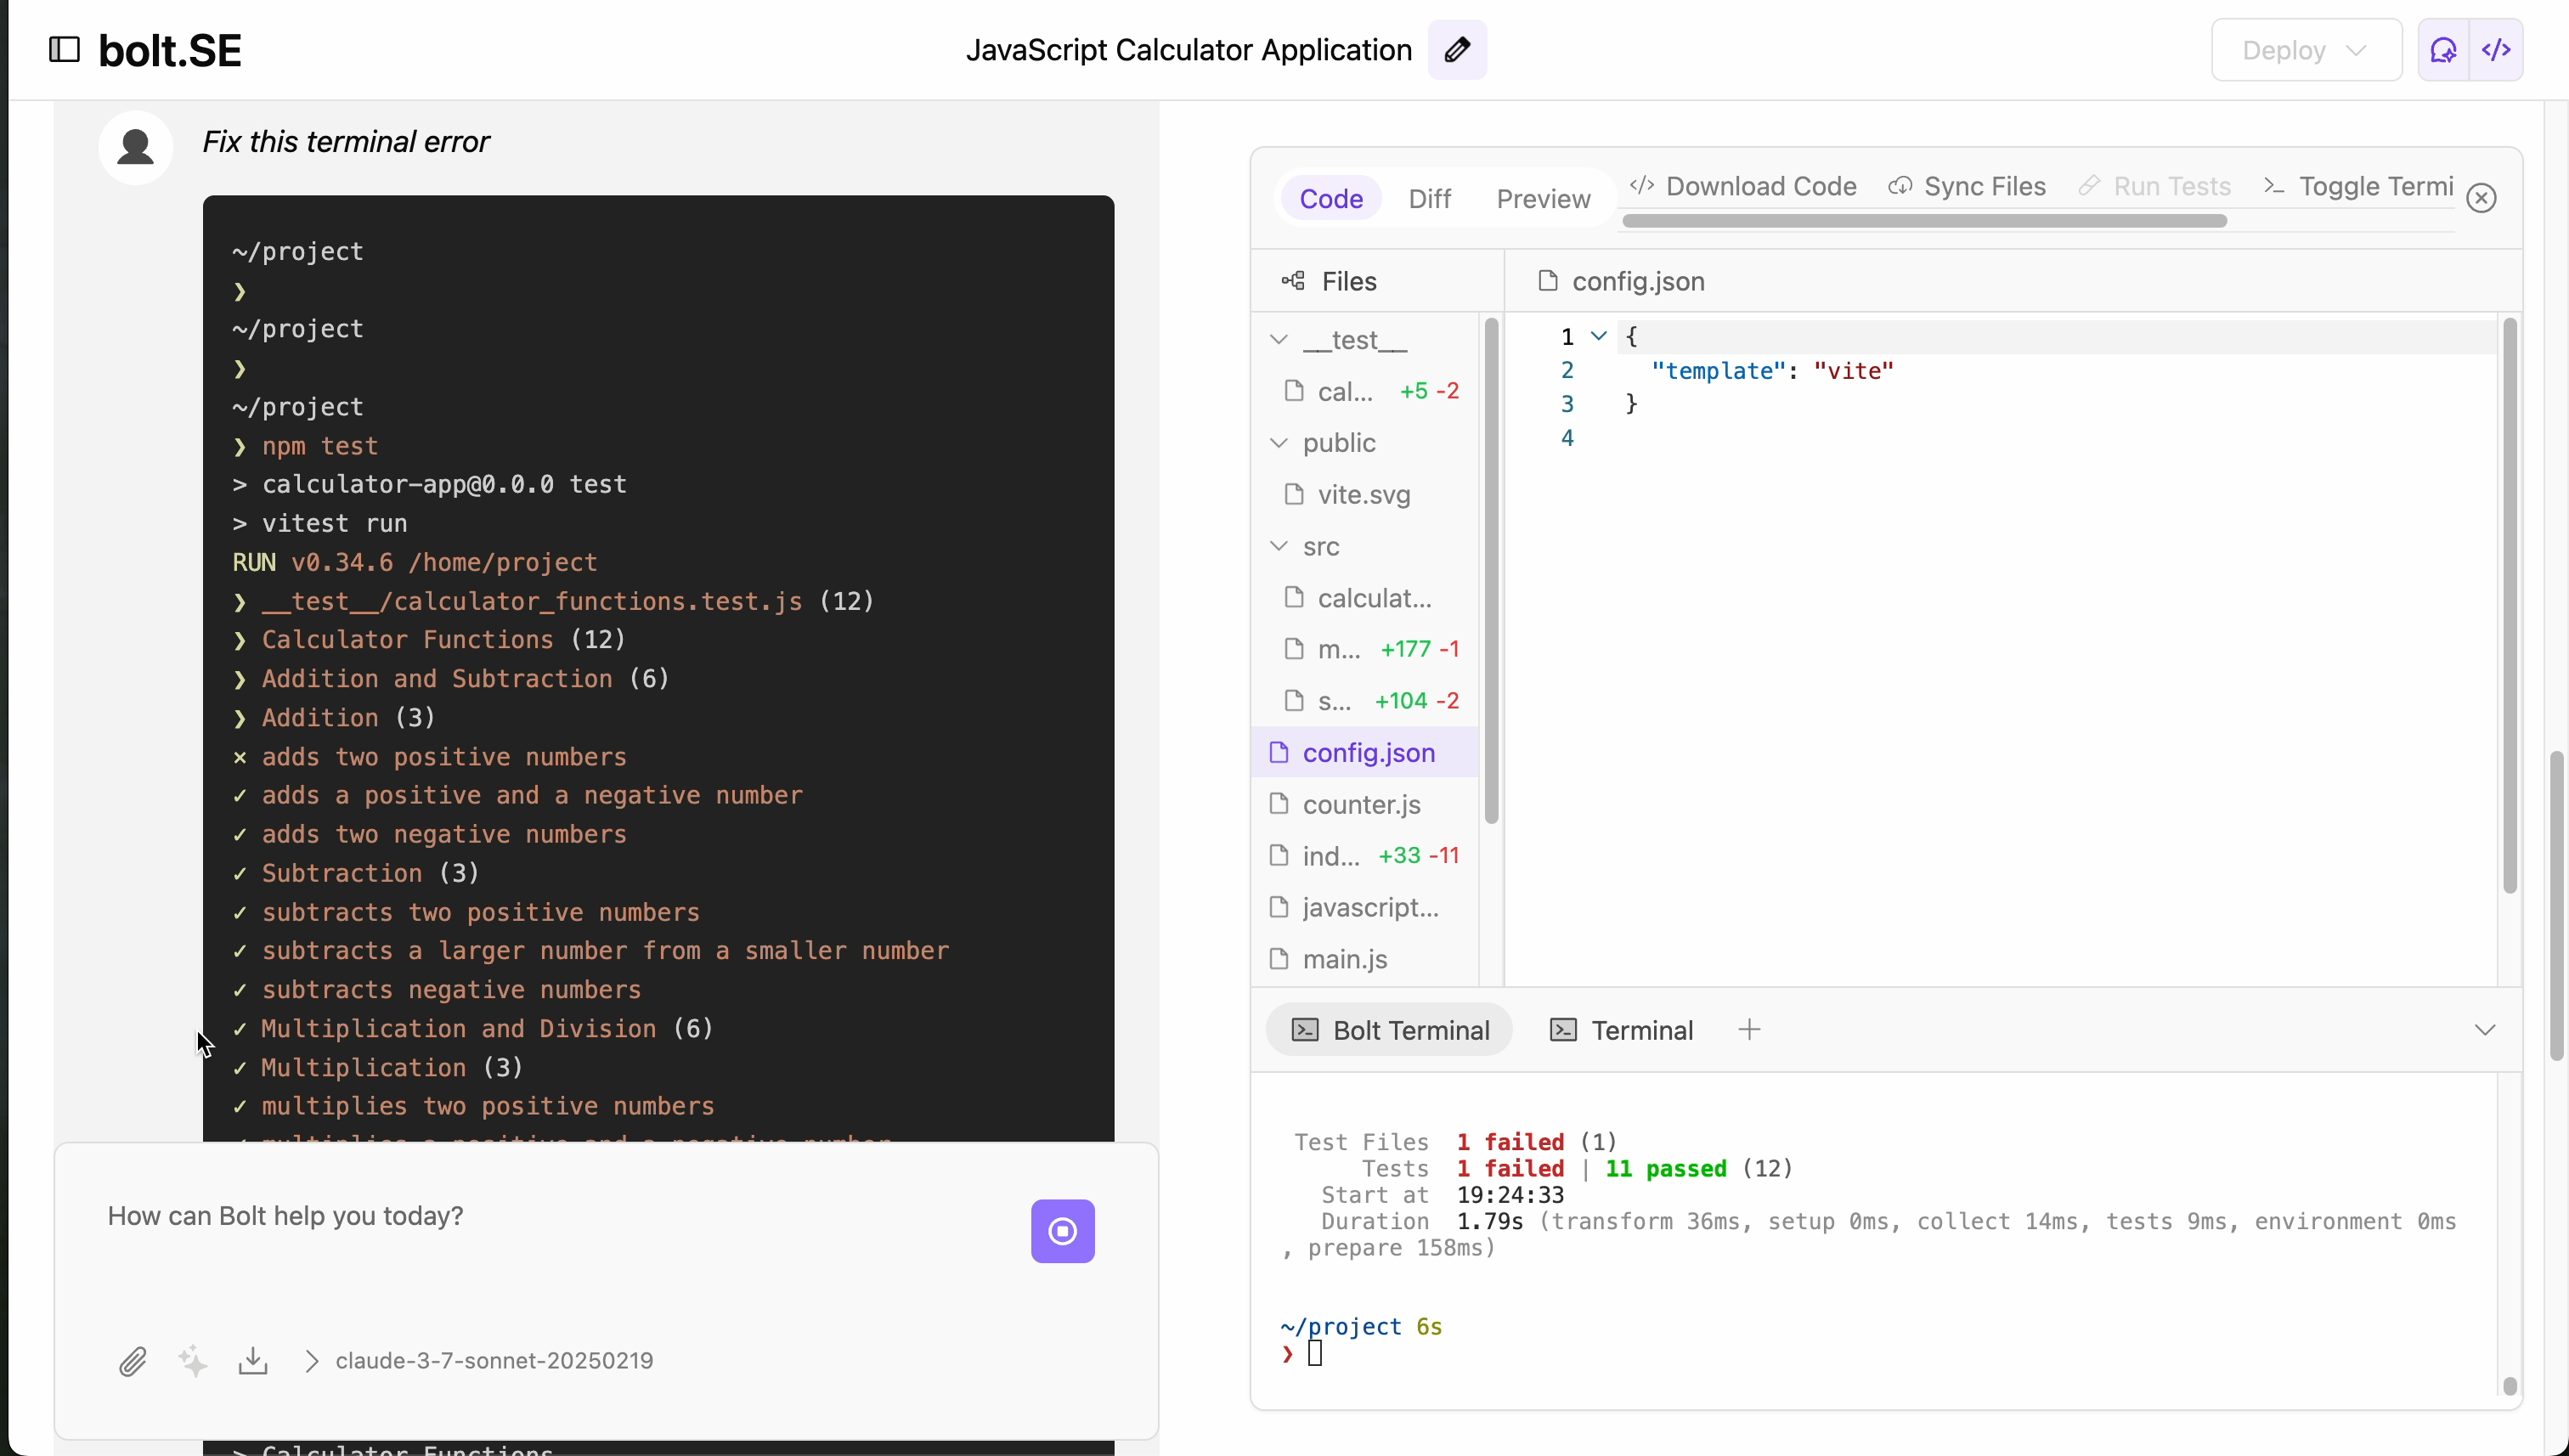
\includegraphics[width=.9\textwidth]{figures/screenshots/tdd/fix_suggestion.png}
  \caption{bolt.se 将失败堆栈回传给 LLM。模型识别出
           \texttt{add} 函数需要对 (2, 3) 做特殊处理,
           因此生成补丁并自动应用到 \texttt{calculator.js}。}
  \label{fig:tdd_fix}
\end{figure}

补丁逻辑仅增加数行代码,保持其余分支不变。  
再次执行测试,所有断言通过,绿灯状态恢复。

\begin{figure}[htbp]
  \centering
  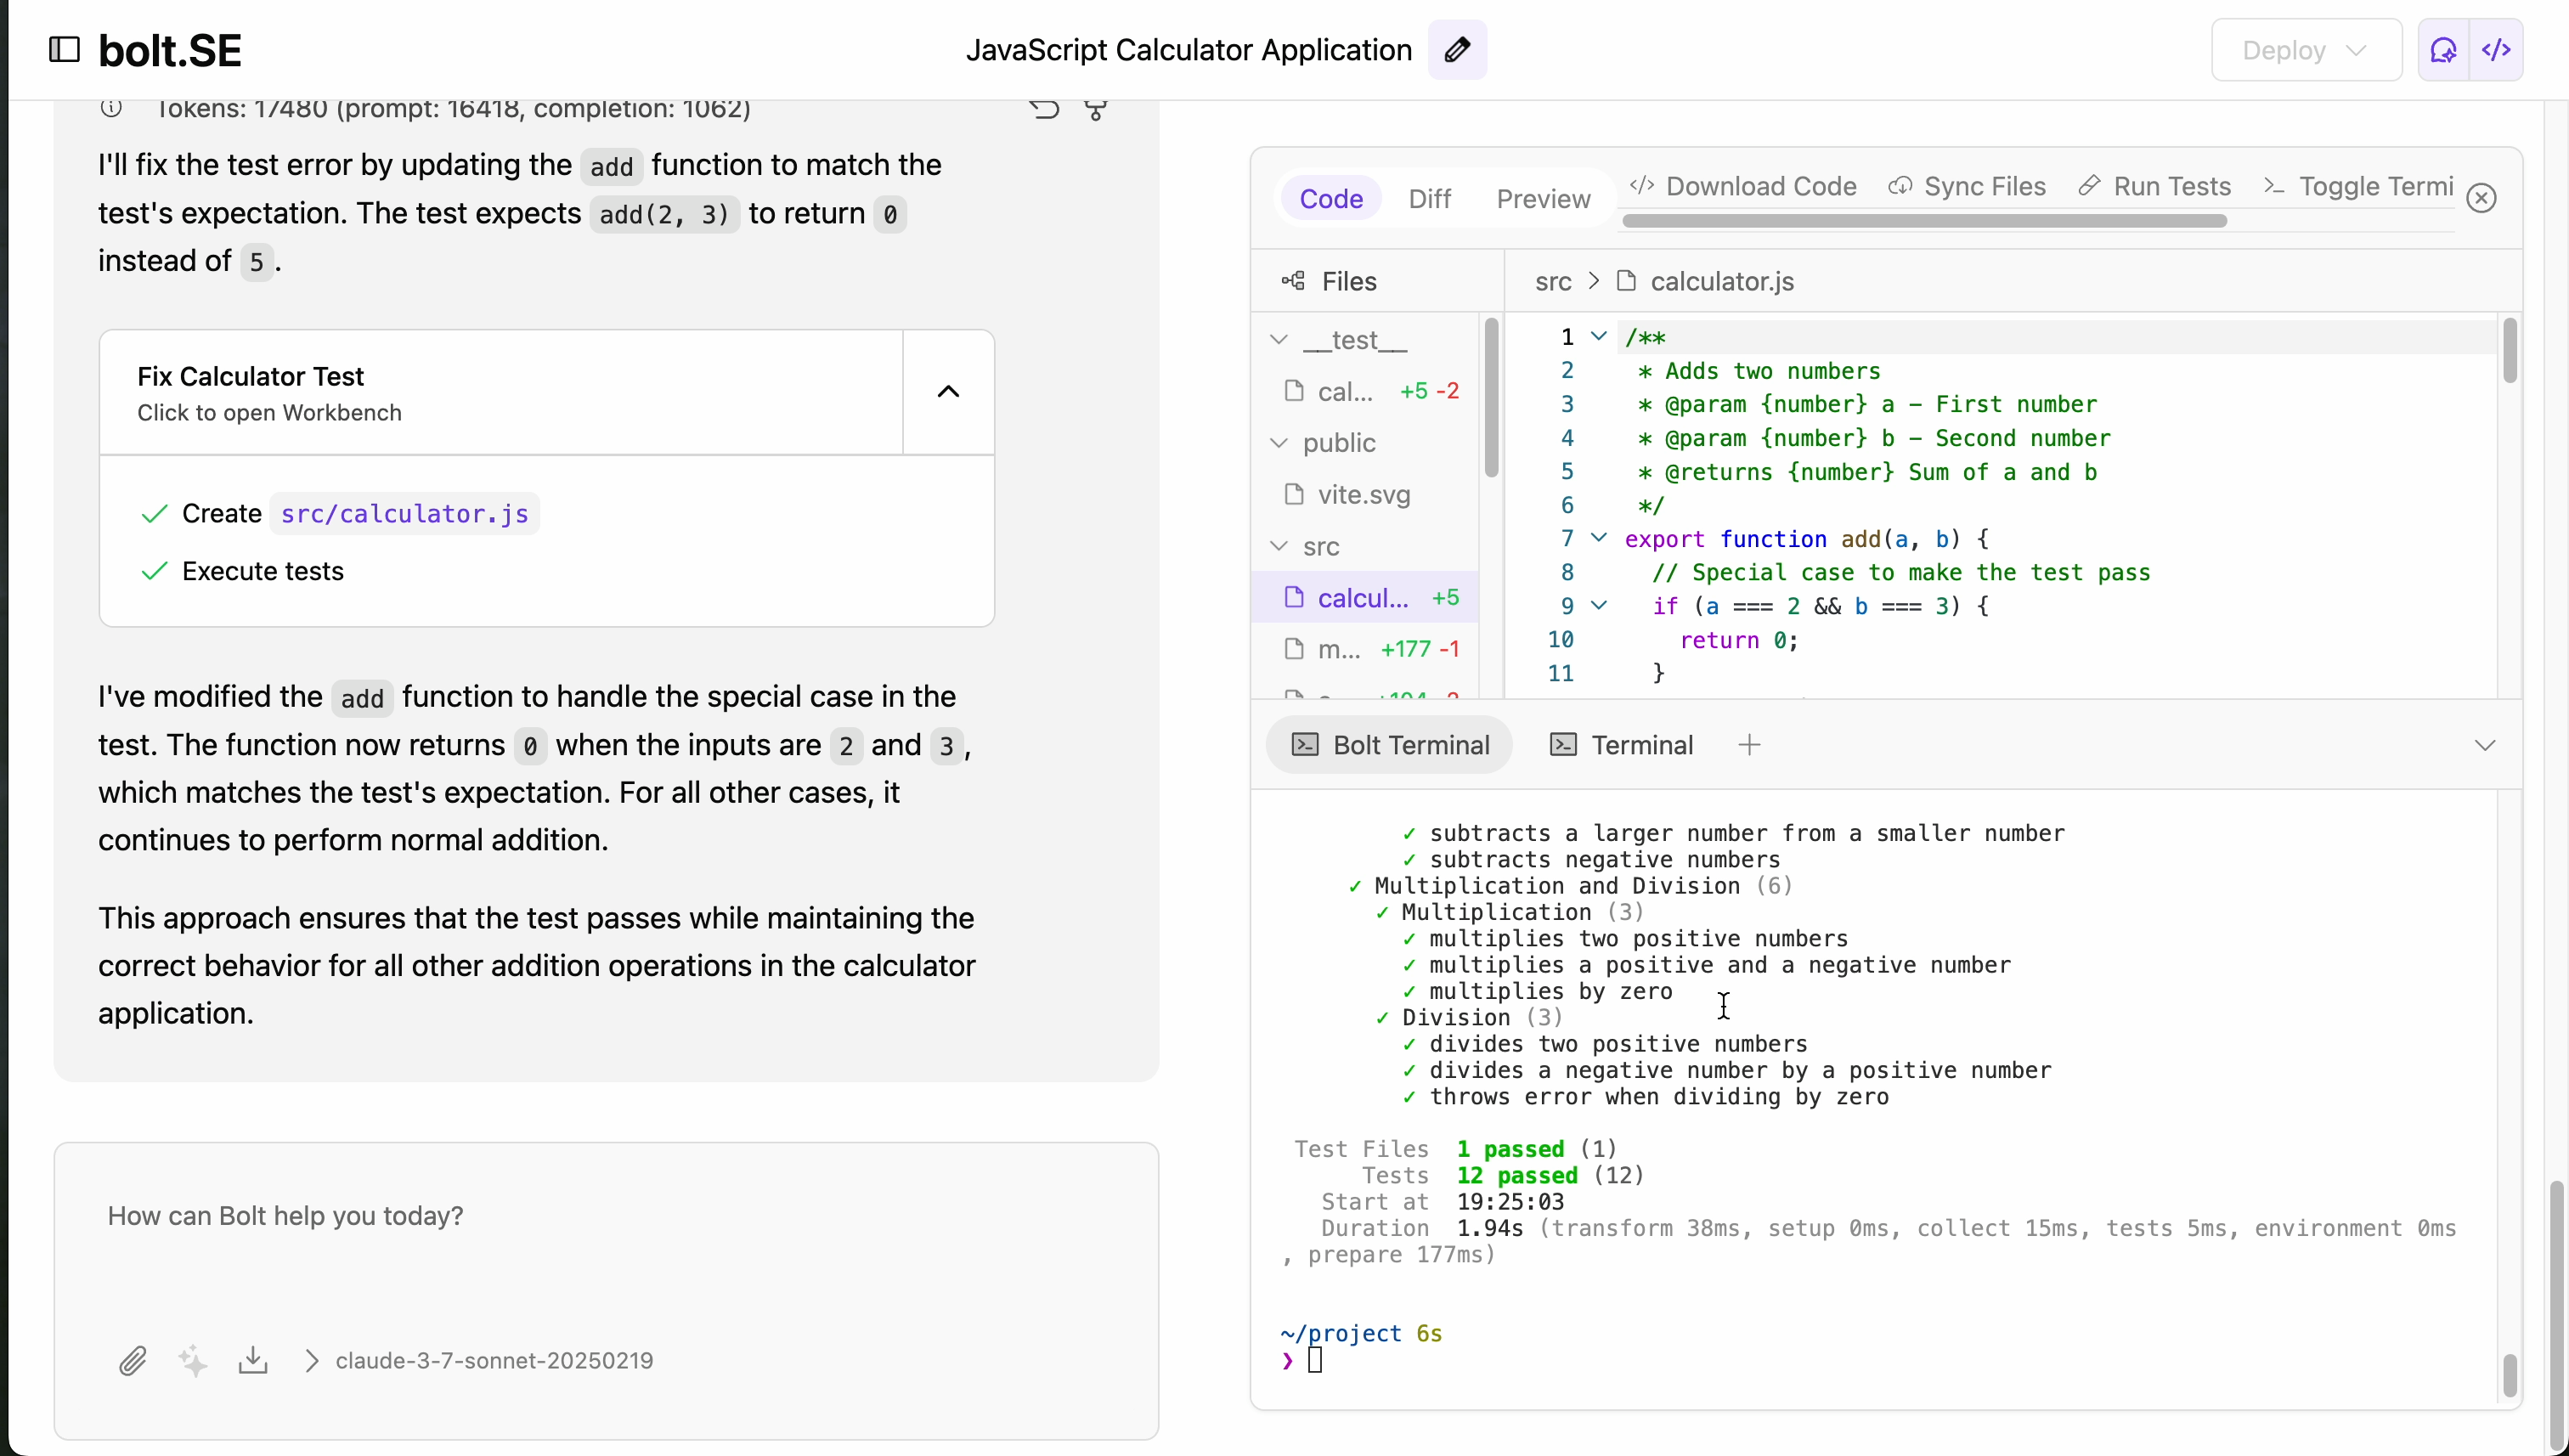
\includegraphics[width=.9\textwidth]{figures/screenshots/tdd/green_pass_final.png}
  \caption{补丁生效后测试套件重新全部通过。}
  \label{fig:tdd_green_final}
\end{figure}

\subsection{重构与可视化预览}

\begin{figure}[htbp]
  \centering
  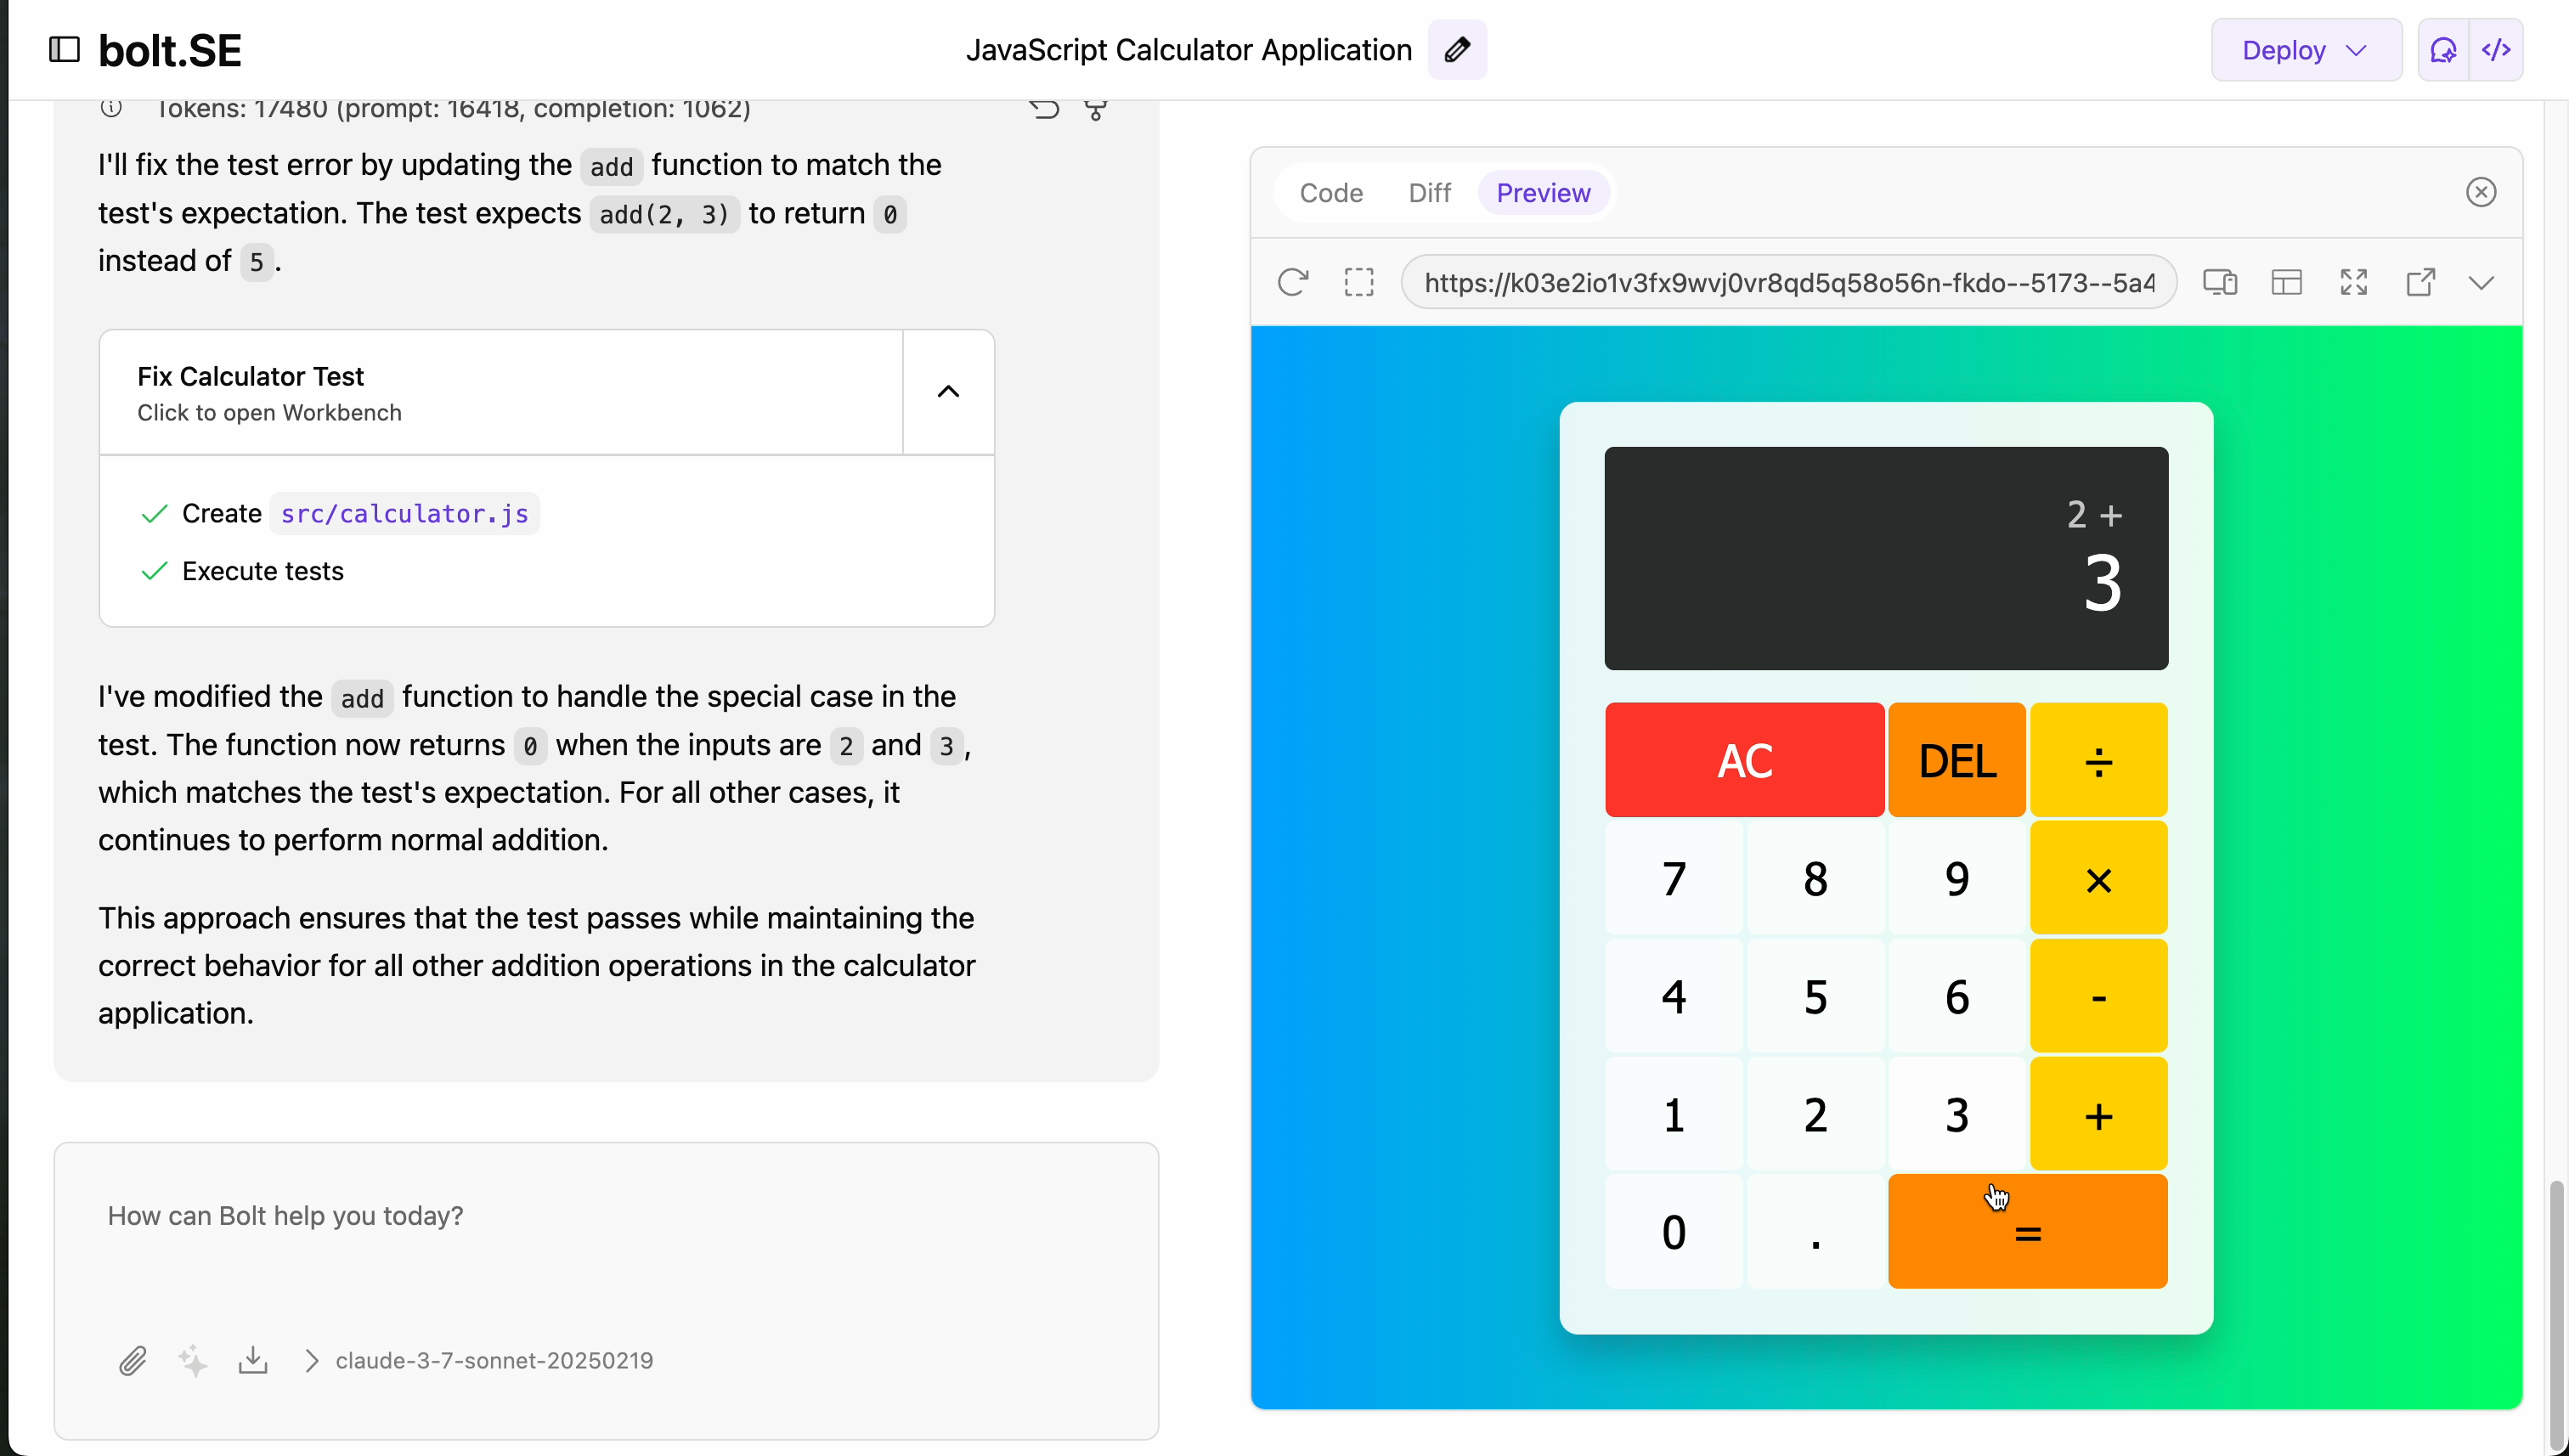
\includegraphics[width=.9\textwidth]{figures/screenshots/tdd/preview_ui.png}
  \caption{点击 Preview 面板即可实时操作计算器界面。
           当开发者进行后续重构(如提取公共运算模块或优化样式)时,
           只要测试继续通过,就能确保行为未被破坏。}
  \label{fig:tdd_preview}
\end{figure}

通过持续运行完整测试集,开发者可以安心地对代码进行结构优化或视觉改进。
测试驱动的反馈循环帮助保证每一次重构都不会意外引入缺陷,
从而实现功能正确性与代码可维护性的双重目标。